% % !Mode:: "TeX:UTF-8"
% \baselineskip 20pt

% %\chapter{个性化显著性评估驱动的评论摘要生成}
% \chapter{基于贝叶斯模型的动态网络层次演化建模(考虑异质性)}
% \label{chap4}
% 上一章介绍了基于决策树的社团转移因素探究框架,通过$15$个真实数据集的分析得到了影响节点社团转移的两个节点的结构属性:节点的度和节点的平均邻居度。受上一章启发,本章认为每个节点的社团转移由于其局部结构不同,都具有不同的转移倾向。而现有的动态网络社团检测模型大部分都将主要的关注点投入到了每个时间快照的社团检测上,而忽略了社团演化,小部分方法如DSBM~\cite{yang2011detecting}虽然关注了社团演化,但是其仅仅通过社团转移矩阵$A$来刻画社团级别的演化,而忽略了同一个社团内的每个节点的社团转移倾向的异质性,也就是说,在DSBM中,其假设同一个社团内的节点在下一个时刻发生转移的趋势都是一样的,且这种趋势在某个固定的社团内是一直不变的。这种假设在本文看来是不合理的。因此本章将会介绍引入更细粒度社团转移趋势的动态网络社团检测生成模型HB-DSBM。
% \section{引言}

% 基于概率模型的社团检测方法,尤其是基于随机块模型(SBM)的方法在动态网络社团检测中具有独特的地位。概率模型通过建立动态复杂网络的生成机制,将社团检测问题转化成了模型的参数估计问题,利用数据拟合模型参数,从而构建出完整的概率模型。利用这种方法进行动态网络社团检测的优点是,模型的任何参数都是可解释的,因此模型中的社团的形成机制也是可以解释的,这就使得人们可以通过概率模型对网络以及社团的生成以及演变过程具有更深层次的理解。而基于随机块模型的社团检测算法就是基于概率模型进行社团检测的算法中的重要一类算法。随机块模型最初的提出是用来解决静态网络社团检测问题,其具有三个基本假设:
% \begin{itemize}
% 	\item 网络中的社团个数是固定的;
% 	\item 每个节点只属于一个社团,且节点之间属于哪个社团是相互独立同分布的;
% 	\item 网络中的两个节点之间有边的概率只与其所在的社团有关。
% \end{itemize}
% 这些假设将网络的生成与社团相结合,从而使得利用生成模型进行社团检测成为可能。而在$2011$年,有人改进了随机块模型,引入了社团演化矩阵,将随机块模型扩展为动态随机块模型(DSBM)。动态随机块模型在动态社团检测中也具有不俗的效果,但是依然存在很多不合理的地方,限制了其社团检测结果。如社团个数固定的假设等,也有很多人对DSBM进行了改进,但是鲜有人注意到DSBM关于社团演化假设的不合理性。DSBM假设了节点的社团转移在所有时间片都是一致的,且只与所在社团有关,这显然是不合理的。本文即在此提出了层次贝叶斯结构重新刻画了节点的社团转移倾向概率。

% 受上一章的启发,本章假设动态网络中同一个社团的不同节点在社团转移行为上具有不同的倾向性,这是由不同节点在社团内具有不同的局部结构决定的。因此本文构建了生成模型HB-DSBM,引入了节点的社团转移倾向参数$C$来刻画每个节点的社团转移倾向。HB-DSBM根据概率图模型对动态网络进行建模,其特点是可以通过对网络的生成机制以及社团的产生机制进行推断并建模,将社团检测这一聚类问题转化为了模型的参数估计问题。而缺点是由于模型较复杂,传统的采样方法较慢,并不能适应大规模数据集,因此本章对HB-DSBM的求解使用了变分推断的方法,结合随机采样能够大大提高模型参数估计的效率。

% \section{HB-DSBM模型构建}

% \subsection{符号表示}
% \begin{table}
% 	\centering
% 	\caption{HB-DSBM模型的符号表示}\label{tab.4.1}
% 	\begin{tabular}{cc}
% 		\hline
% 		{\bfseries 符号} &  { \bfseries 描述} \\
% 		\hline
% 		$K$,$N$,$T$ & 分别为社团个数、节点数和时间快照数 \\
% 		\hline
% 		$W^{t}$ & $t$时间快照对应的邻接矩阵\\
% 		\hline
% 		$\pi_k$ & 在时间快照$1$中,$i$节点属于社团$k$的概率\\
% 		$z_i^{t}$ & 在$t$快照中,$i$节点属于哪个社团 \\
% 		${A}_k$ & $k$社团的社团级别转移倾向 \\
% 		${C}_i^{t}$ & $i$节点在$t$快照中的节点级别转移倾向, 其中$t=2, \cdots, T$,$i=1, \cdots, N$\\
% 		$B_{kl}$ & 属于$k$社团的节点与属于$l$社团的节点在任意时间快照中的连边概率\\
% 		\hline
% 		${\gamma}$ ,${\mu}$ & ${\pi}$和${A}_k$的狄利克雷分布参数 \\
% 		${\alpha}$ , ${\beta}$ & $B$的Beta分布的参数 \\   
% 		\hline
% 	\end{tabular}
% \end{table}

% 在介绍模型前,本章首先介绍模型的符号表示。如表\ref{tab.4.1}所示,本章用$W=\{W^1,W^2,...,W^T\}$表示动态网络邻接矩阵,即$W^t$表示第$t$个网络快照的邻接矩阵,其中$t \in 1,...,T$。这里$W^t \in \{0,1\}^{N\times N}$,其中$W_{ij}^t = 0$则代表$i$节点与$j$节点在网络快照$t$中没有边,若为$1$则有边。这里为了方便叙述,本章认为网络是无向无权的,这里需要说明,HB-DSBM可以有效的扩展为有向有权网络。$Z = \{Z^1,Z^2,...,Z^T\}$代表每个网络快照中节点的社团划分,例如$z_i^t = k$则表示$i$节点在网络快照$t$中属于$k$社团,其中$k\in K$。

% \subsection{HB-DSBM模型}

% \begin{figure}[!htbp]
% 	\setlength{\abovecaptionskip}{0pt} 
% 	\setlength{\belowcaptionskip}{10pt} 
% 	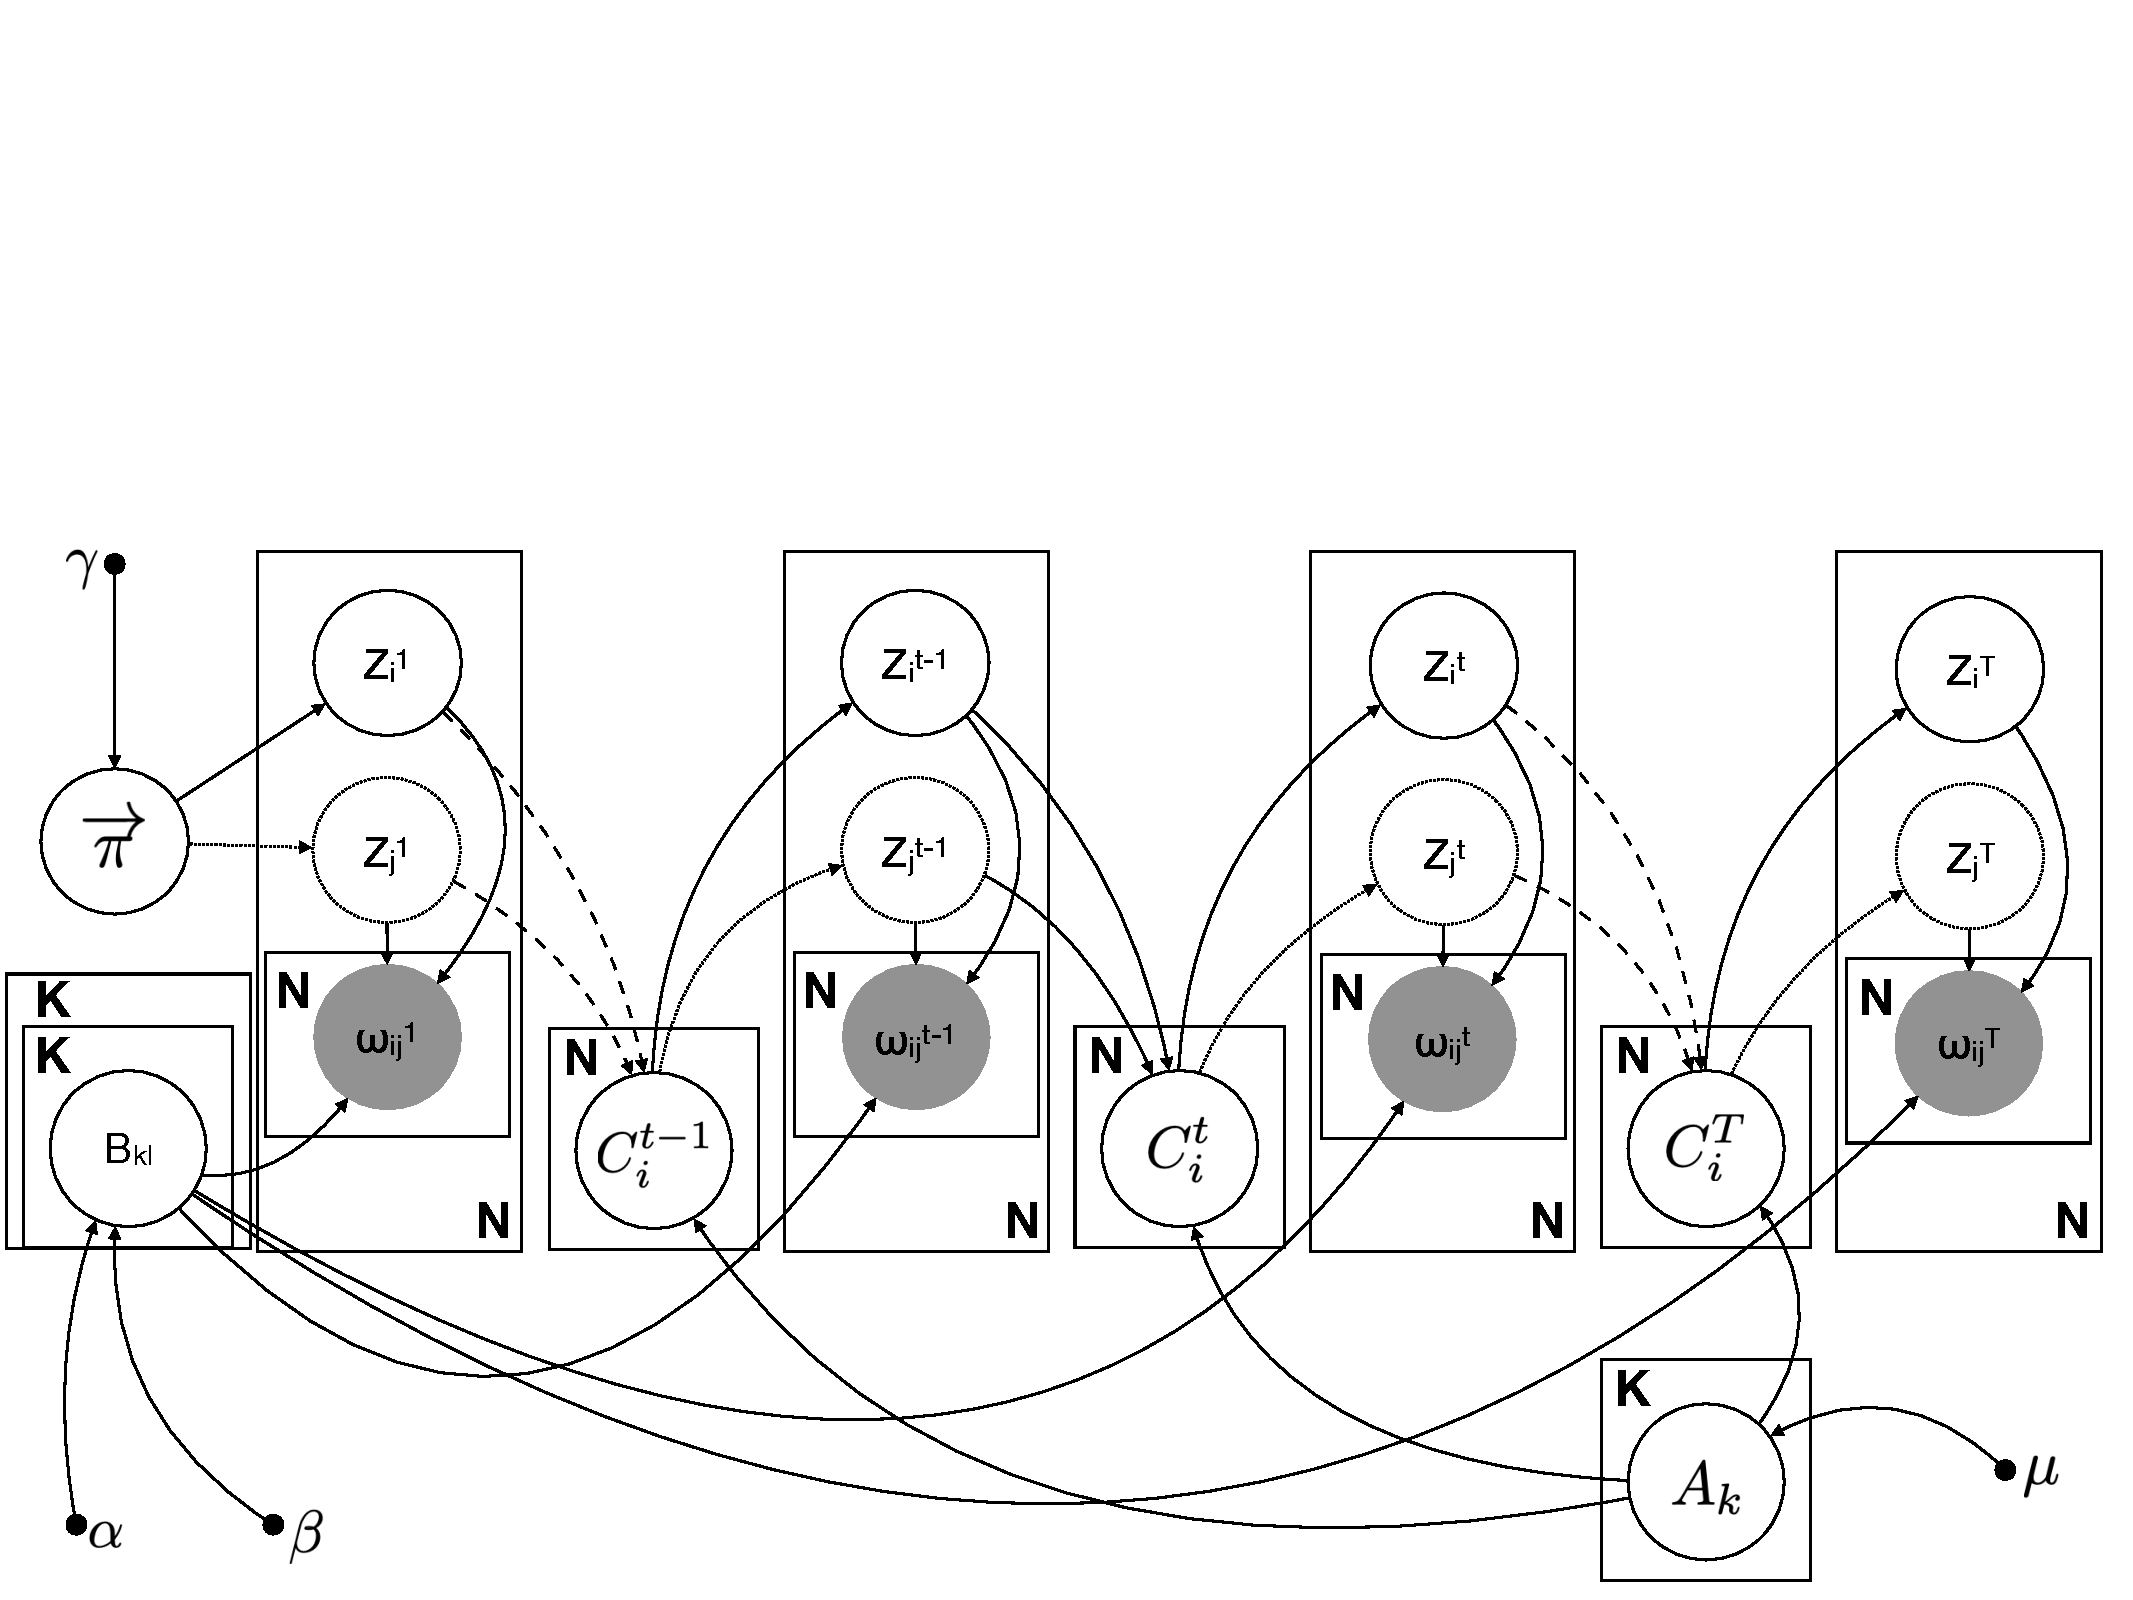
\includegraphics[width=.9\textwidth]{figures/chap04/graph-model_v3_cuted.pdf}
% 	\caption{HB-DSBM图模型}
% 	\label{fig.4.1}
% \end{figure}

% 本节首先介绍HB-DSBM的核心生成机制来揭示它是如何通过层次贝叶斯结构同时建模社团级别和节点级别的动态演化的,随后给出其产生社团结构和动态网络的生成过程。

% 如图~\ref{fig.4.1}的图模型所示,HB-DSBM首先令$\pi$表示$Z^1$的先验分布,同时$\pi$服从参数为$\gamma$的狄利克雷分布。$B$是不同社团间节点的连边概率,即类随机块模型中的块矩阵,例如$B_{kl}$即代表属于$k$社团和属于$l$社团的节点之间连边的概率。而$B$服从参数为$\alpha$和$\beta$的Beta分布。

% 本章中的$A \in [0, 1]^{K \times K}$表示社团级别转移倾向矩阵,$A$的每一行$A_k$都服从参数为$\mu$的狄利克雷分布,因此 $\sum_l A_{kl} = 1$。同时$C = \{ C^2, \cdots C^T \}$表示节点级别的社团转移倾向,每个$C^t$都是由社团级别转移倾向矩阵$A$生成。对于$t>1$的网络快照,任意节点$i$都有其唯一的转移向量 $C_i^t  \in [0, 1]^K$,该向量服从以参数为$A_{z_i^{t-1}}$的狄利克雷分布,因此$\sum_{k} C_{ik}^t = 1$。这一部分就是本模型的核心:层次狄利克雷生成机制。

% 基于以上机制,模型就可以生成社团标签以及动态网络中每个网络快照中的边。具体生成过程如下所示:
% \begin{enumerate}
% 	\item 生成初始社团划分概率 ${\pi} \sim Dir({\gamma})$
% 	\item 生成块矩阵 $B \sim Beta({\alpha},{\beta})$
% 	\item 对于网络快照$t=1$的每个节点$i$:
% 	\begin{enumerate}
% 		\item 生成每个节点的社团归属 $z_i^1 \sim Mult({\pi})$ 
% 		\item 生成每条边 $\omega_{ij}^1 \sim Bernoulli(\cdot | B_{z_i^1,z_j^1})$
% 	\end{enumerate}
% 	\item 生成每个社团级别转移矩阵的社团转移向量 ${A}_k \sim Dir({\mu})$
% 	\item 对网络快照$t>1$中的每个节点$i$:
% 	\begin{enumerate}
% 		\item 生成每个节点级别的社团转移向量${C}_i^t \sim Dir({A}_{z_i^{t-1}})$
% 		\item 生成每个节点的社团归属 $z_i^t \sim Mult({C}_i^t)$
% 		\item 生成每条边 $\omega_{ij}^t \sim Bernoulli(\cdot | B_{z_i^t,z_j^t})$
% 	\end{enumerate}
% \end{enumerate}

% 由生成过程可知,当$t=1$时,模型首先利用参数为$\pi$的多项分布生成$i$的社团归属$z_i^1$,随后以伯努利分布 $Bernoulli(\cdot|B_{z_i^1,z_j^1})$生成每对节点对$i,j$之间的连边。而当$t>1$时,$i$节点的社团归属由以参数为$C_i^t$的多项分布决定,即$z_i^t \sim Mult({C}_i^t)$。而$C_i^t$服从狄利克雷分布$Dir(A_{z_i^{t-1}})$。

% 根据如图~\ref{fig.4.1}的概率图模型和生成过程,可以写出HB-DSBM的联合概率分布如下:

% \begin{equation}
% \begin{split}
% Pr&(W_T,Z_T,C_T,B,A,\pi|\alpha,\beta,\gamma,\mu) \\
% = & \prod_{t=1}^T Pr(W^t | Z^t,B) Pr(Z^1|\pi) \prod_{t=2}^T Pr(Z^t|C^t) \\
% & \prod_{t=2}^T Pr(C^t|A,Z^{t-1}) Pr(A|\mu) Pr(\pi|\gamma) Pr(B|\alpha,\beta) \\
% \end{split}
% \end{equation}

% \section{模型求解}

% 本小结介绍针对本模型的高效的变分近似推断算法。
% \subsection{变分推断}
% 由于模型参数较多且复杂,直接推出模型后验$p(Z,C,B,A,\pi|W)$是困难的, 因此基于平均场理论,本节提出了用$q(Z,C,B,A,\pi)$ 来近似$p(Z,C,B,A,\pi|W)$. 为了简介,本节用$\Delta$ 来表示参数 $\{\pi,B,A,C,Z\}$. 更详细来说,即:

% \begin{equation}
% \label{eq2}
% \begin{split}
% & q(\Delta) =  \prod_{t=1}^T \prod_{i=1}^N q(z_i^t) \prod_{t=2}^T \prod_{i=1}^N q(c_i^t)q(B)q(A)q(\pi)  \\
% \end{split}
% \end{equation}

% 其中块矩阵变分参数$q(B|\widetilde{\alpha},\widetilde{\beta}) = \prod_{k,l\geq k} Beta(\widetilde{\alpha}_{kl},\widetilde{\beta}_{kl})$, 社团级别转移矩阵变分参数 $q(A|\widetilde{\mu}) = \prod_{k=1}^K \prod_{l=1}^K Dir(\widetilde{\mu}_{kl})$。 而社团归属变分参数$q(z_i^t|\widetilde{\phi}_i^t)$ 服从以$\widetilde{\phi}_i^t$为参数的多项分布。
% 而$q(c_i^t|\widetilde{\xi}_i^t)$和$q(\pi|\widetilde{\gamma})$都分别服从以$\widetilde{\xi}_i^t$和$\widetilde{\mu}_{kl}$为参数的狄利克雷分布。

% 因此有变分下界:
% %  \begin{equation}
% %  \begin{split}
% %     % & q(z_i^t|\widetilde{\phi}_i^t) \sim Multi(\widetilde{\phi}_i^t)\\
% %     % & q(c_i^t|\widetilde{\xi}_i^t) \sim Dir(\widetilde{\xi}_i^t)\\
% %     % & q(B|\widetilde{\alpha},\widetilde{\beta}) = \prod_{k,l\geq k} q(B_{kl}|\widetilde{\alpha}_{kl},\widetilde{\beta}_{kl})\\
% %     % & q(B_{kl}|\widetilde{\alpha}_{kl},\widetilde{\beta}_{kl}) = Beta(\widetilde{\alpha}_{kl},\widetilde{\beta}_{kl}) \\
% %     & q(B|\widetilde{\alpha},\widetilde{\beta}) = \prod_{k,l\geq k} Beta(\widetilde{\alpha}_{kl},\widetilde{\beta}_{kl}) \\
% %     & q(A|\widetilde{\mu}) = \prod_{k=1}^K \prod_{l=1}^K Dir(\widetilde{\mu}_{kl}) \\
% %     % & q(A|\widetilde{\mu}) = \prod_{k=1}^K \prod_{l=1}^K q(A_{kl} | \widetilde{\mu}_{kl})\\
% %     % & q(A_{kl} | \widetilde{\mu}_{kl}) \sim Dir(\widetilde{\mu}_{kl})\\
% %     % & q(\pi|\widetilde{\gamma}) = Dir(\widetilde{\gamma})\\
% %  \end{split}
% %  \end{equation}

% \begin{equation}
% \label{eq:3}
% \begin{split}
% &\widetilde{L}(q) = \sum_z \int_{\pi,B,A,C}q(\Delta) \log \frac{p(\Delta,W)}{q(\Delta)} 
% %  \end{split}
% %  \end{equation}
% %  By considering the constant
% %  \begin{equation}
% %  \begin{split}
% %      \widetilde{L}(q) = \log p(\pi,B,A,C,Z,W) - KL(q||p)
% %  \end{split}
% %  \end{equation}
% %  
% %  The ELBO is given by:
% %  \begin{equation}
% %  \begin{split}
% = E_{\widetilde{\phi},\widetilde{\alpha},\widetilde{\beta}} \sum_{t=1}^T [\log P(W^t|Z^t,B)] \\
% &+ E_{\widetilde{\gamma},\widetilde{\phi}}[\log P(Z^1|\pi)]+E_{\widetilde{\phi},\widetilde{\xi}} \sum_{t=2}^T [\log P(Z^t|C^t)] 
% + E_{\widetilde{\xi},\widetilde{\phi},\widetilde{\mu}} \sum_{t=2}^T [\log P(C^t|A,Z^{t-1})]\\
% &+ E_{\widetilde{\mu}}[\log P(A)]+E_{\widetilde{\gamma}}[\log P(\pi)] + E_{\widetilde{\alpha},\widetilde{\beta}}[\log P(B)]
% - E_{\widetilde{\gamma}}[\log q(\pi)] - E_{\widetilde{\alpha},\widetilde{\beta}}[\log q(B)]  - E_{\widetilde{\mu}}[\log q(A)]\\
% &- \sum_{t=2}^T \sum_{i=1}^N E_{\widetilde{\xi}}[\log q(C_i^t)] - \sum_{t=1}^T \sum_{i=1}^N E_{\widetilde{\phi}}[\log q(z_i^t)] \\
% \end{split}
% \end{equation}

% 这里 $\widetilde{\phi},\widetilde{\xi},\widetilde{\alpha},\widetilde{\beta},\widetilde{\mu},\widetilde{\gamma}$ 即为变分参数。为了方便起见,本章省略掉了分布的条件部分。 例如,本章将 $q(\Delta|\widetilde{\phi},\widetilde{\xi},\widetilde{\alpha},\widetilde{\beta},\widetilde{\mu},\widetilde{\gamma})$ 和 $q(z_i^t|\widetilde{\phi}_i^t)$ 略写为$q(\Delta)$和$q(z_i^t)$。
% 因此该模型的变分下界(ELBO)$\widetilde{L}(q)$被写成了如上式\ref{eq:3}。

% 随后通过最大化ELBO来获得最优的隐变量$Z,\pi,B,A,C$和模型参数$\gamma,\alpha,\beta,\mu$。 通过对不同的参数$\widetilde{\phi},\widetilde{\gamma},\widetilde{\alpha},\widetilde{\beta},\widetilde{\mu},\widetilde{\xi}$对$\widetilde{L}(q)$求偏导,并令导数为0求得每个参数的更新公式,即:
% \begin{equation}
% \begin{split}
% \nabla \widetilde{L}(q) = \{ \frac{\partial \widetilde{L}}{\partial \widetilde{\gamma}},\frac{\partial \widetilde{L}}{\partial \widetilde{\alpha}},\frac{\partial \widetilde{L}}{\partial \widetilde{\beta}},\frac{\partial \widetilde{L}}{\partial \widetilde{\mu}},\frac{\partial \widetilde{L}}{\partial \widetilde{\xi}},\frac{\partial \widetilde{L}}{\partial \widetilde{\phi}} \} = 0
% \end{split}
% \end{equation}

% 每个参数的结果如下所示:
% \textbf{对 $\widetilde{\gamma}$}:

% 包含$\widetilde{\gamma}$的ELBO如下所示:
% \begin{equation}
% \begin{split}
% & \widetilde{L}_{\widetilde{\gamma}} = E_{\widetilde{\gamma},\widetilde{\phi}}[\log P(Z^1|\pi)] + E_{\widetilde{\gamma}}[\log P(\pi)]- E_{\widetilde{\gamma}}[\log q(\pi)] \\
% & = \log{\frac{\prod_{k=1}^K \log \Gamma (\widetilde{\gamma}_k)}{\Gamma (\sum_k \widetilde{\gamma}_k)}} 
%  + \sum_{k=1}^K ( \gamma_k - \widetilde{\gamma}_k + \sum_{i=1}^N \widetilde{\phi}_{ik}^1)[\psi(\widetilde{\gamma}_k) - \psi(\sum_k \widetilde{\gamma}_k)]\\
% \end{split}
% \end{equation}

% 这里 $\psi(x) = \frac{\Gamma'(x)}{\Gamma(x)} = \frac{\,d \log \Gamma(x)}{\, dx}$. 
% 通过对$\widetilde{L}_{\widetilde{\gamma}}$ 针对$\widetilde{\gamma}$求偏导,并令导数等于0,得到其更新公式如下:
% \begin{equation}
% \label{eq4}
% \begin{split}
% \widetilde{\gamma}_k = \gamma_k + \sum_{i=1}^N \widetilde{\phi}_{ik}^1, \quad
% % \widetilde{\mu}_{kl} \propto \mu_l + \frac{\sum_{t=2}^T \sum_i \widetilde{\phi}_{ik}^{t-1}}{T-1}
% \end{split}
% \end{equation}

% \textbf{对于$\widetilde{\xi}$}:

% ELBO中包含$\widetilde{\xi}$的式子如下所示:
% \begin{equation}
% \begin{split}
% &\widetilde{L}_{\widetilde{\xi}} = E_{\widetilde{\phi},\widetilde{\xi}} \sum_{t=2}^T [\log P(Z^t|C^t)] 
% + E_{\widetilde{\xi},\widetilde{\phi},\widetilde{\mu}} \sum_{t=2}^T [\log P(C^t|A,Z^{t-1})] - \sum_{t=2}^T \sum_{i=1}^N E_{\widetilde{\xi}}[\log q(C_i^t)]\\
% \end{split}
% \end{equation}

% 利用同样方法求得更新公式如下所示:

% \begin{equation}
% \label{eq5}
% \begin{split}
% \widetilde{\xi}_{ik}^t \propto \widetilde{\phi}_{ik}^t + \sum_l \widetilde{\phi}_{il}^{t-1}(\frac{\widetilde{\mu}_{kl}}{\sum_l \widetilde{\mu}_{kl}} - 1) + 1
% \end{split}
% \end{equation}

% \textbf{对于参数$\widetilde{\alpha}$和$\widetilde{\beta}$}:

% ElBO中包含$\widetilde{\alpha}$和$\widetilde{\beta}$的式子如下所示:
% \begin{equation}
% \begin{split}
% &\widetilde{L}_{\widetilde{\alpha},\widetilde{\beta}} = E_{\widetilde{\phi},\widetilde{\alpha},\widetilde{\beta}} \sum_{t=1}^T [\log P(W^t|Z^t,B)] 
% - E_{\widetilde{\alpha},\widetilde{\beta}}[\log q(B)] + E_{\widetilde{\alpha},\widetilde{\beta}}[\log P(B)]\\
% &= \sum_{k \leq l} \log\{\frac{\Gamma(\widetilde{\alpha}_{kl})\Gamma(\widetilde{\beta}_{kl})}{\Gamma(\widetilde{\alpha}_{kl}+\widetilde{\beta}_{kl})}   \}  \\
% &+ \sum_{k=1}^K [\alpha_{kk}- \widetilde{\alpha}_{kk} +\sum_t \sum_{i < j} \widetilde{\phi}_{ik}^t\widetilde{\phi}_{jk}^t w_{ij}^t]
% [\psi(\widetilde{\alpha}_{kk})-\psi (\widetilde{\alpha}_{kk}+\widetilde{\beta}_{kk})] \\
% &+ \sum_{k=1}^K [\beta_{kk}- \widetilde{\beta}_{kk} +\sum_t \sum_{i < j} \widetilde{\phi}_{ik}^t\widetilde{\phi}_{jk}^t(1- w_{ij}^t)]
% [\psi(\widetilde{\beta}_{kk})-\psi (\widetilde{\alpha}_{kk}+\widetilde{\beta}_{kk})] \\
% &+ \sum_{k<l}^K [\alpha_{kl}- \widetilde{\alpha}_{kl} +\sum_t \sum_{i \neq j} \widetilde{\phi}_{ik}^t\widetilde{\phi}_{jk}^t w_{ij}^t]
% [\psi(\widetilde{\alpha}_{kl})-\psi (\widetilde{\alpha}_{kl}+\widetilde{\beta}_{kl})] \\
% &+ \sum_{k<l}^K [\beta_{kl}- \widetilde{\beta}_{kl} +\sum_t \sum_{i \neq j} \widetilde{\phi}_{ik}^t\widetilde{\phi}_{jk}^t(1- w_{ij}^t)]
% [\psi(\widetilde{\beta}_{kl})-\psi (\widetilde{\alpha}_{kl}+\widetilde{\beta}_{kl})] \\
% \end{split}
% \end{equation}

% 利用同样方法求得$\widetilde{\alpha}$和$\widetilde{\beta}$的更新公式如下:

% \begin{equation}
% \label{eq6}
% \begin{split}
% & \widetilde{\alpha}_{kk} = \alpha_{kk} + \frac{\sum_t \sum_{i<j} \widetilde{\phi}_{ik}^t \widetilde{\phi}_{jk}^t w_{ij}^t}{T}  \\
% & \widetilde{\beta}_{kk} = \beta_{kk} + \frac{\sum_t \sum_{i<j} \widetilde{\phi}_{ik}^t \widetilde{\phi}_{jk}^t (1-w_{ij}^t)}{T} \\
% & \widetilde{\alpha}_{kl} = \alpha_{kl} + \frac{\sum_t \sum_{i \neq j} \widetilde{\phi}_{ik}^t \widetilde{\phi}_{jl}^t w_{ij}^t}{T} \\
% & \widetilde{\beta}_{kl} = \beta_{kl} + \frac{\sum_t \sum_{i \neq j} \widetilde{\phi}_{ik}^t \widetilde{\phi}_{jl}^t (1-w_{ij}^t)}{T}  \\
% \end{split}
% \end{equation}

% \textbf{对于 $\widetilde{\mu}$}:

% ELBO中包含$\widetilde{\mu}$的式子如下所示:

% \begin{equation}
% \begin{split}
% & \widetilde{L}_{\widetilde{\mu}} = E_{\widetilde{\xi},\widetilde{\phi},\widetilde{\mu}} \sum_{t=2}^T [\log P(C^t|A,Z^{t-1})] 
% - E_{\widetilde{\mu}}[\log q(A)]+ E_{\widetilde{\mu}}[\log P(A)]\\
% &=\sum_{t=2}^T \sum_i \sum_k \sum_l \widetilde{\phi}_{ik}^{t-1} [\sum_l \psi(\widetilde{\mu}_{kl}) - \psi(\sum_l \widetilde{\mu}_{kl}) 
% + \frac{\widetilde{\mu}_{kl}}{\sum_l \widetilde{\mu}_{kl}}(\psi(\widetilde{\xi}_{ik}^t)-\psi(\sum_l \widetilde{\xi}_{il}^t))]  \\
% &-\log[\Gamma(\sum_l \widetilde{\mu}_{kl})] + \sum_l \log[\Gamma(\widetilde{\mu}_{kl})]
% + \sum_l (\mu_l - \widetilde{\mu}_{kl})[\psi(\widetilde{\mu}_{kl}) - \psi(\sum_l \widetilde{\mu}_{kl})]  \\
% \end{split}
% \end{equation}

% 因此有:
% \begin{equation}
% \label{eq7}
% \begin{split}
% \widetilde{\mu}_{kl} \propto \mu_l + \frac{\sum_{t=2}^T \sum_i \widetilde{\phi}_{ik}^{t-1}}{T-1}
% \end{split}
% \end{equation}

% \textbf{对于 $\widetilde{\phi}$}:

% $\widetilde{\phi}$ 是社团划分参数$Z$的变分参数,其更新公式随$t$的不同而不同。下面分情况讨论:

% \textbf{当$t=1$时}:

% ELBO中包含$\widetilde{\phi}$的项并考虑约束$\sum_k \widetilde{\phi}_{ik} = 1$,有:

% \begin{equation}
% \begin{split}
% &\widetilde{L}_{\widetilde{\phi}} = E_{\widetilde{\phi},\widetilde{\alpha},\widetilde{\beta}} [\log P(W^1|Z^1,B)] + E_{\widetilde{\gamma},\widetilde{\phi}}[\log P(Z^1|\pi)] \\
% &+ E_{\widetilde{\xi},\widetilde{\phi},\widetilde{\mu}}[\log P(C^2|A,Z^1)] - E_{\widetilde{\phi}}[\log q(Z^1)]+\rho (\sum_k \widetilde{\phi}_{ik}-1)\\
% \end{split}
% \end{equation}

% 因此有:

% %Here $\phi$ is the variational parameter of $Z$ with $T$ snapshot, we get the update rules of $\phi$ at different snapshots $t$ as follows.
% %When $t=1$:
% \begin{equation}
% \label{eq8}
% \begin{split}
% &\widetilde{\phi}_{ik}^1 \propto \exp\{\sum_j \sum_l \widetilde{\phi}_{jl}^1 [w_{ij}^1[\psi(\widetilde{\alpha}_{kl})-\psi(\widetilde{\alpha}_{kl}+\widetilde{\beta}_{kl})]
%   + (1-w_{ij}^1)[\psi(\widetilde{\beta}_{kl}) - \psi(\widetilde{\alpha}_{kl}+\widetilde{\beta}_{kl})] ]   \\
% & +[\psi(\widetilde{\gamma}_k)-\psi(\sum_l \widetilde{\gamma}_l) ] +[\sum_l \psi(\widetilde{\mu}_{kl}) - \psi(\sum_l \widetilde{\mu}_{kl}) 
% + \sum_l (\frac{\widetilde{\mu}_{kl}}{\sum_l \widetilde{\mu}_{kl}}-1)(\psi (\widetilde{\xi}_{ik}^2) - \psi(\sum_l \widetilde{\xi}_{il}^2))]  \} \\
% \end{split}
% \end{equation}

% \textbf{当$1<t<T$}:

% ELBO中包含$\widetilde{\phi}$的项,同时考虑$\sum_k \widetilde{\phi}_{ik} = 1 $,有:

% \begin{equation}
% \begin{split}
% & \widetilde{L}_{\widetilde{\phi}} = E_{\widetilde{\phi},\widetilde{\alpha},\widetilde{\beta}} [\log P(W^t|Z^t,B)]+E_{\widetilde{\phi},\widetilde{\xi}} [\log P(Z^t|C^t)]\\
% &+  E_{\widetilde{\xi},\widetilde{\phi},\widetilde{\mu}} [\log P(C^{t+1}|A,Z^t)]- \sum_{i=1}^N E_{\widetilde{\phi}}[\log q(z_i^t)]\\
% \end{split}
% \end{equation}
% %When $1<t<T$:
% 因此有:
% \begin{equation}
% \label{eq9}
% \begin{split}
% &\widetilde{\phi}_{ik}^t \propto \exp \{ \sum_j \sum_l \widetilde{\phi}_{jl}^t [w_{ij}^t[\psi(\widetilde{\alpha}_{kl}) - \psi(\widetilde{\alpha}_{kl}+\widetilde{\beta}_{kl})]
% + (1-w_{ij}^t)[\psi(\widetilde{\beta}_{kl})-\psi(\widetilde{\alpha}_{kl}+\widetilde{\beta}_{kl})]]    \\
% & + [\psi(\widetilde{\xi}_{ik}^t) - \psi(\sum_l \widetilde{\xi}_{il}^t)]+ [\sum_l \psi(\widetilde{\mu}_{kl}) - \psi(\sum_l \widetilde{\mu}_{kl}) 
% +\sum_l (\frac{\widetilde{\mu}_{kl}}{\sum_l \widetilde{\mu}_{kl}} -1)(\psi(\widetilde{\xi}_{ik}^{t+1}) - \psi(\sum_l \widetilde{\xi}_{il}^{t+1}))]  \}\\
% \end{split}
% \end{equation} 

% \textbf{当$t=T$}:

% ELBO中包含$\widetilde{\phi}$的项同时考虑约束$\sum_k \widetilde{\phi}_{ik} = 1 $,有:

% \begin{equation}
% \begin{split}
% & \widetilde{L}_{\widetilde{\phi}} = E_{\widetilde{\phi},\widetilde{\alpha},\widetilde{\beta}} [\log P(W^T|Z^T,B)]+E_{\widetilde{\phi},\widetilde{\xi}} [\log P(Z^T|C^T)]
% - \sum_{i=1}^N E_{\widetilde{\phi}}[\log q(z_i^T)]\\
% \end{split}
% \end{equation}
% %   When $t=T$:
% 因此有:
% \begin{equation}
% \label{eq10}
% \begin{split}
% &\widetilde{\phi}_{ik}^T \propto \exp \{ \sum_j \sum_l \widetilde{\phi}_{jl}^T [w_{ij}^T[\psi(\widetilde{\alpha}_{kl}) - \psi(\widetilde{\alpha}_{kl}+\widetilde{\beta}_{kl})] + \\
% &(1-w_{ij}^T)[\psi(\widetilde{\beta}_{kl})-\psi(\widetilde{\alpha}_{kl}+\widetilde{\beta}_{kl})]]  + [\psi(\widetilde{\xi}_{ik}^T) - \psi(\sum_l \widetilde{\xi}_{il}^T)]\}  \\
% \end{split}
% \end{equation} 
% % Here $\psi(x) = \frac{\Gamma'(x)}{\Gamma(x)} = \frac{\,d \log \Gamma(x)}{\, dx}$. 

% 由更新公式可知,模型超参数$\mu$和$\alpha$ 都为常量且其不影响模型结果。下面介绍得到更新公式后的迭代算法

% \subsection{迭代算法}

% 现在已经有了所有参数的更新公式,下面给出变分EM的更新算法如算法~\ref{alg4.1}所示。

% \begin{algorithm}
% 	\caption{HB-DSBM迭代算法}\label{alg4.1}
% 	\algorithmicrequire ~~ 动态网络邻接矩阵 $W$, 对大迭代次数 $n_{max}$ 和阈值变量$\varepsilon$ \\
% 	\algorithmicensure ~~ $\widetilde{\alpha},\widetilde{\beta},\widetilde{\gamma},\widetilde{\mu},\widetilde{\xi},\widetilde{\phi}$
% 	\begin{algorithmic}[1]
% 		\REPEAT
% 		\STATE 给定$\widetilde{\phi}$, 根据迭代公式~\ref{eq4}
% 		~\ref{eq5}~\ref{eq6}~\ref{eq7}更新 $\widetilde{\xi},\widetilde{\gamma},\widetilde{\alpha},\widetilde{\beta},\widetilde{\mu}$
% 		\STATE 给定 $\widetilde{\xi},\widetilde{\gamma},\widetilde{\alpha},\widetilde{\beta},\widetilde{\mu}$, 根据迭代公式\ref{eq8}~\ref{eq9}~\ref{eq10}更新 $\widetilde{\phi}$ 
% 		\UNTIL {$|\mathcal{L}^{new}-\mathcal{L}^{old}|<\varepsilon$ 或迭代次数 $> n_{max}$}
% 		\RETURN $\widetilde{\xi},\widetilde{\gamma},\widetilde{\alpha},\widetilde{\beta},\widetilde{\mu},\widetilde{\phi}$
% 	\end{algorithmic}
% \end{algorithm}

% 算法的复杂度依赖于三个部分。 更新$\phi$的复杂度是$O(TN^2K^2)$, 其中 $T$ 是网络快照的个数,  $N$ 网络中节点的数量,而$K$ 是社团的个数。 而更新 $\xi$的复杂度是$O(TNK^2)$。 最后ELBO的计算复杂度是$O(TN^2K^2)$.因此理论上该算法的复杂度是 $O(N^2)$. 而真实世界网络的数据往往是稀疏的,因此可以通过负采样或并行计算有效提升算法的运行效率,使其适应于大规模数据集。

% \section{实验及验证}

% 本小节将本文提出的算法HB-DSBM与四种同类动态网络社团检测算法在四个数据集(两个生成数据集与两个真实数据集)进行比较,以证明HB-DSBM的效果优于同类方法。同时在DBLP数据集中对HB-DSBM与DSBM进行社团演化分析,以证明本方法的社团演化分析更加细致且符合实际。
% \subsection{数据集}
% 本章实验使用四个数据集对HB-DSBM及对比方法进行比较,包括两个生成数据集和两个真实数据集,所有数据集均有真相。

% \textbf{data1} 由Lin 等人~\cite{lin2008facetnet}基于Girvan 和Newman提出的数据的改进版数据集。该数据集具有不同的参数设置,每个参数设置组生成的数据包含$10$个时间快照和$128$个节点,这些节点分别属于$4$个不同的社团,每个社团均包含32个节点。参数$\sigma$表示某社团内部的节点与其他社团的节点连边的数量的均值;而$nC$代表每个时间快照到下一个时间快照离开其原有社团的节点的数量;$aD$则表示每个节点的平均度。

% \textbf{data2}是由Greene等人\cite{greene2010tracking}提出的。该数据集融合了社团级别的事件使得其更接近真实世界数据,该数据集中的每个网络包含$1000$个节点,$15$的平均度和$50$的最大节点度。该数据集的社团个数有$20$到$50$不等,社团间连边的概率为$0.2$。值得一提的是,该数据集中的节点服从网络的power-law。

% \textbf{KIT-email}\cite{gorkedynamic}数据集是email收发网络,其节点代表电子邮箱账号。本文将该数据集视作无向无权网络,并将该数据集处理成网络快照形式的数据,分别以$2$或$3$个月为一个时间间隔。其节点数以及社团个数对应于这两个时间间隔分别为$138$、$170$和$23$、$25$。

% \textbf{DBLP}\cite{konect:2017:dblp-cite}数据是开源的论文数据集。本文选取了涉及计算机的三个领域的数据,包括数据挖掘(DM)、数据库(DB)和人工智能(AI)。时间跨度为$9$年,其中包括$1163$个节点和按领域划分的$3$个社团。本文将数据划分为$9$个网络快照,每个快照对应一年。

% \subsection{动态社团检测}
% 本小结社团检测实验选取了四种动态网络社团检测方法,分别为DSBM~\cite{yang2011detecting}、DYNMOGA~\cite{folino2014evolutionary}、Genlouvain~\cite{jutla2011generalized}和PisCES~\cite{liu2018global},这四种动态社团检测方法均为不同实现方式得到的高质量的动态网络社团检测算法。以上四个算法的参数设置均遵从其原论文的最优设置。而HB-DSBM的超参数如前文所述,均对模型效果影响不大,因此实验部分设置参数为当$k \neq l$时 $\alpha_{kl} = 1$,而当$k \neq l$时 $\alpha_{kk} = 10$;$\beta$的设置与$\alpha$相同; $\mu$的设置和$\gamma$相同, 即 $\mu_k = \gamma_k = \frac{1}{K}$,其中$1<k<K$。
% \subsubsection{评价指标}
% 本章实验部分使用标准化互信息指标(NMI)~\cite{gong2007machine}作为社团检测效果的评价指标,这也是目前大部分动态社团检测方法所使用的评价指标。NMI被设计为静态网络社团划分的评价指标,因此本章会在每个时间快照计算社团划分的NMI值。NMI被用作网络社团划分衡量指标需要知道网络社团划分的真相。令$C=\{C_1,...,C_K\}$表示网络社团划分的真相,令 $C'=\{C'_1,...,C'_K\}$代表待评估的社团划分,其中$C_k$和$C'_k$分别代表真相以及待评估的第$k$个社团的所有节点。则NMI的定义如下所示:

% \begin{equation}
% \begin{split}
% NMI(C,C')=\frac{\sum_{C,C'}p(C,C')\log \frac{p(C,C')}{p(C)p(C')}}{max(H(C)H(C'))}
% \end{split}
% \end{equation}

% 其中,$H(C)$和$H(C')$表示社团$C$和$C'$的熵。NMI的值在$0$到$1$之间。NMI的值越高,代表待评估的社团划分与真相越接近。



% \subsubsection{实验结果}

% 将HB-DSBM与DYNOMGA、DSBM、GenLou以及PisCES在不同数据集中进行NMI对比。在$data1$不同参数设置中的对比结果如图~\ref{fig.4.2}所示,HB-DSBM在图~\ref{fig.4.2}(a)中比效果最好的DSBM有大约明显的NMI提升,同时在图~\ref{fig.4.2}(d)中有$0.1$的NMI提升。虽然HB-DSBM在图~\ref{fig.4.2}(b)与图~\ref{fig.4.2}(c)中与其余方法的NMI提升差距不大,但是依然是效果最好的。HB-DSBM在五种方法中具有最好的NMI效果,证明该方法正确的把握住了节点演化的模式。HB-DSBM的曲线更加平滑,因为该模型结合了社团级别的演化以及节点级别的演化模式,成功的把握住了节点演化的异质性。DSBM的NMI曲线也比其他方法更加平滑,因为其融合了社团级别的演化模式,但是其忽略了同社团节点内演化模式的异质性。反观DYNOMGA和GenLou将社团检测与社团演化看做了两个独立的部分,因此其NMI曲线不够平滑,特别是在图~\ref{fig.4.2}(c)和图~\ref{fig.4.2}(d)中。而PisCES在不同时间快照中显示了很大的NMI反差,说明其对网络的噪声非常敏感。

% \begin{figure}[htbp]
% 	\centering
% 	\subfigure[$\sigma=4,nC=9,aD=16$]{
% 		\label{Fig.4.2.a}
% 		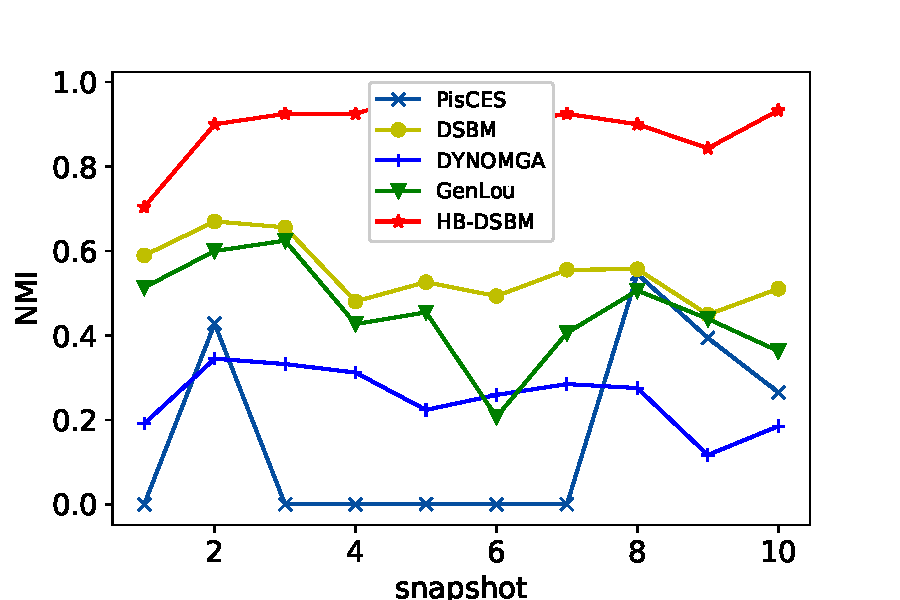
\includegraphics[width=.48\textwidth]{figures/chap04/compare4916.pdf}
% 	}
% 	\subfigure[$\sigma=4,nC=9,aD=20$]{
% 		% \label{Fig.vis.1}
% 		\label{Fig.4.2.b}
% 		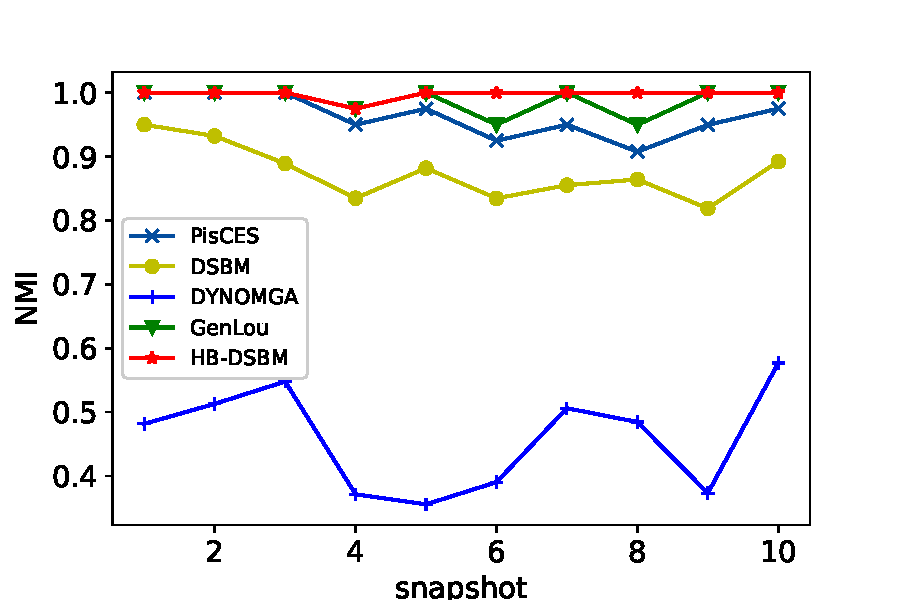
\includegraphics[width=.48\textwidth]{figures/chap04/compare4920.pdf}
% 	}
% 	\subfigure[$\sigma=5,nC=3,aD=16$]{
% 		% \label{Fig.vis.1}
% 		\label{Fig.4.2.c}
% 		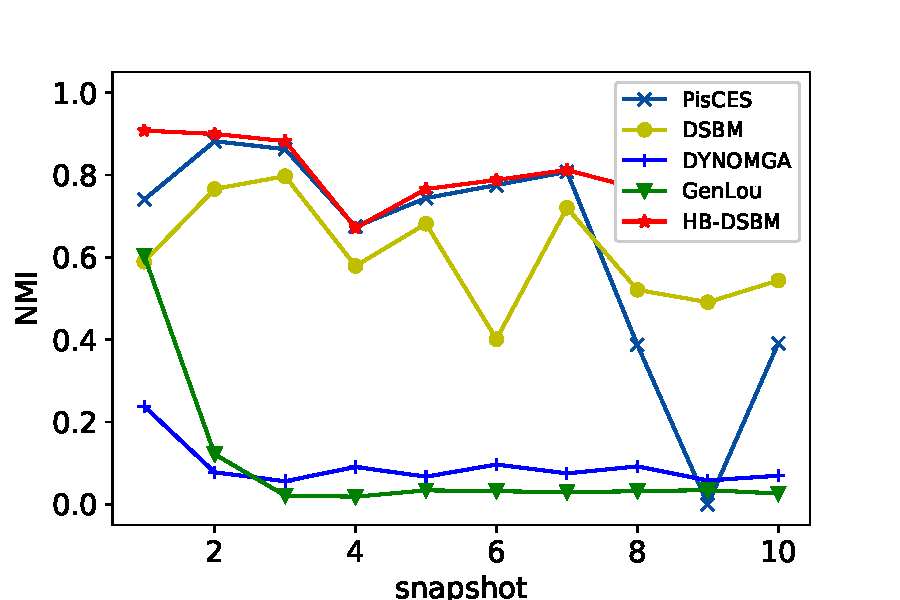
\includegraphics[width=.48\textwidth]{figures/chap04/compare5320.pdf}
% 	}
% 	\subfigure[$\sigma=5,nC=9,aD=20$]{
% 		% \label{Fig.vis.1}
% 		\label{Fig.4.2.d}
% 		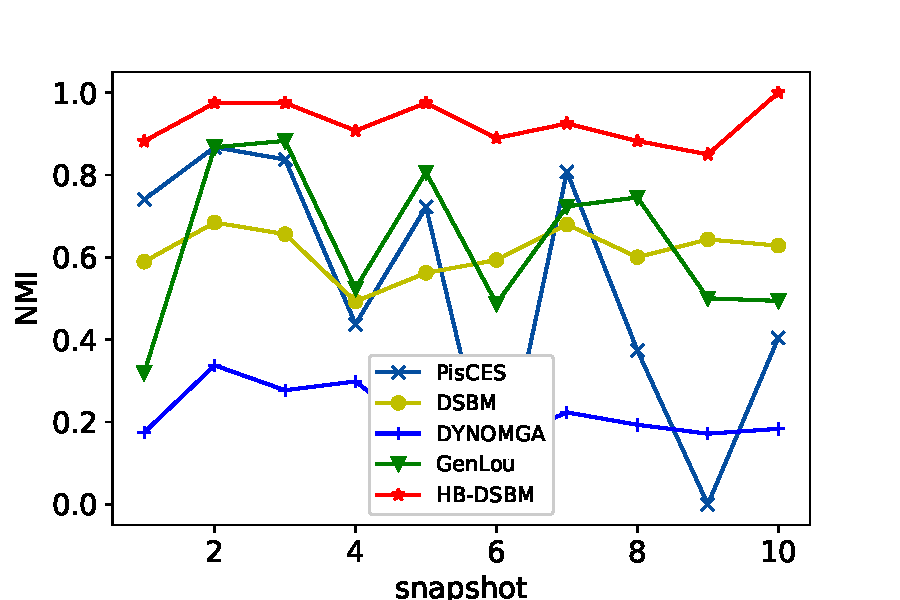
\includegraphics[width=.48\textwidth]{figures/chap04/compare5920.pdf}
% 	}
% 	\caption{$data1$四种不同参数设置的不同方法NMI对比。}
% 	\label{fig.4.2}
% \end{figure}

% 至于$data2$,NMI的结果显示如图~\ref{fig.4.3}所示,HB-DSBM依然具有最好的效果。在该数据集中,PisCES显示出比除HB-DSBM外其他方法更好的效果,而DSBM却显示除了最差的NMI表现,因为其利用吉布斯采样对模型进行求解,使得该模型在大规模数据中的有限次迭代中很难达到局部最优,即使是在每个网络快照$1000$个节点的数据集中。



% \begin{figure}[htbp]
% 	\centering
% 	\subfigure[扩展事件网络]{
% 		% \label{Fig.vis.1}
% 		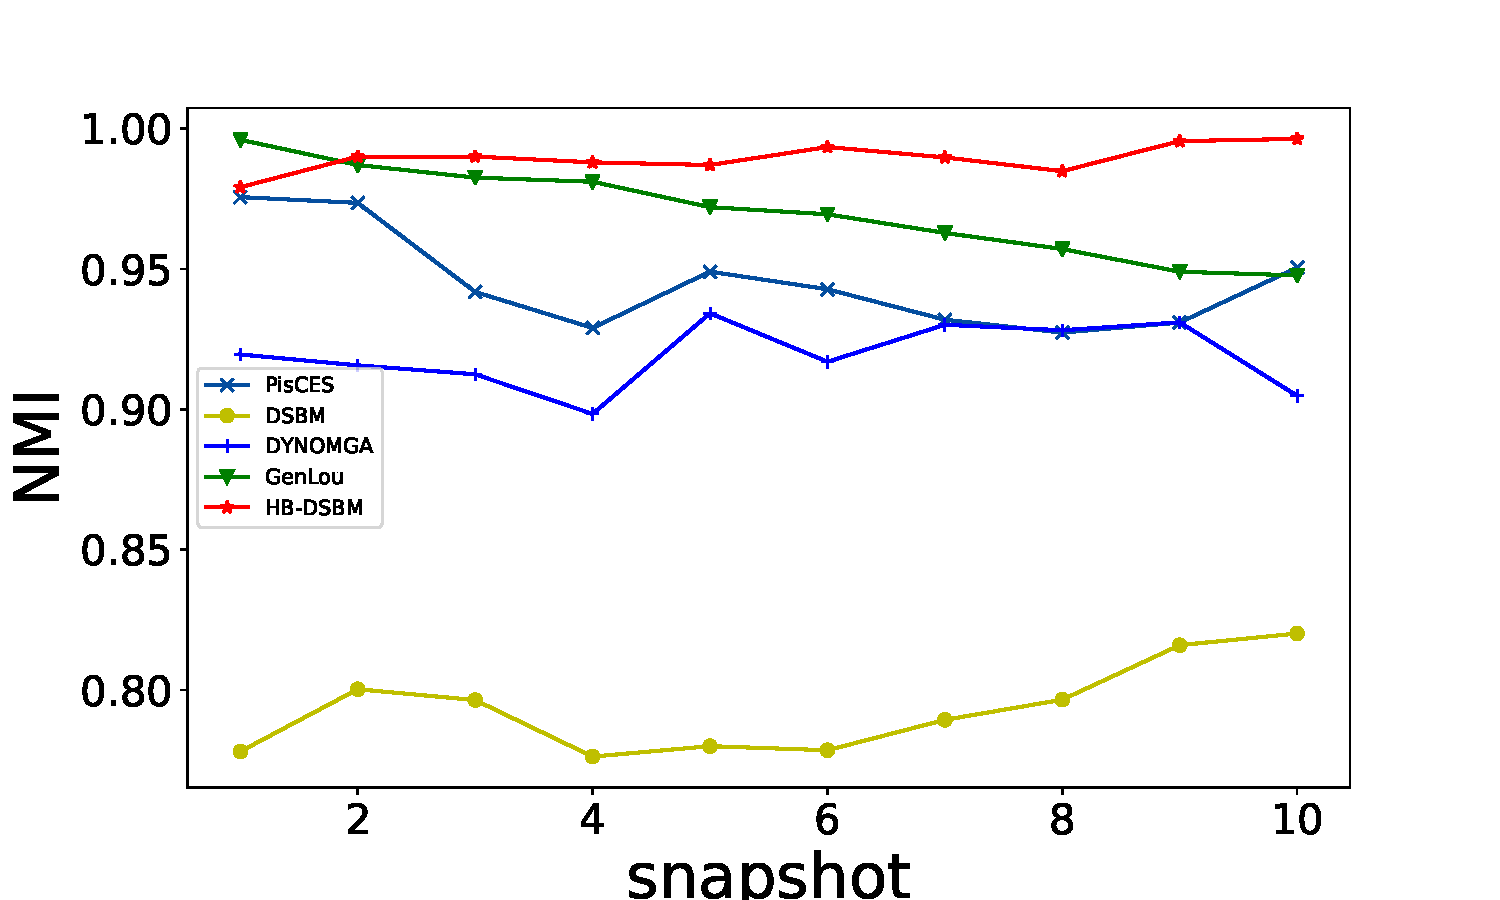
\includegraphics[width=.48\textwidth]{figures/chap04/asonexp11.pdf}}
% 	\subfigure[社团交换事件网络]{
% 		% \label{Fig.vis.1}
% 		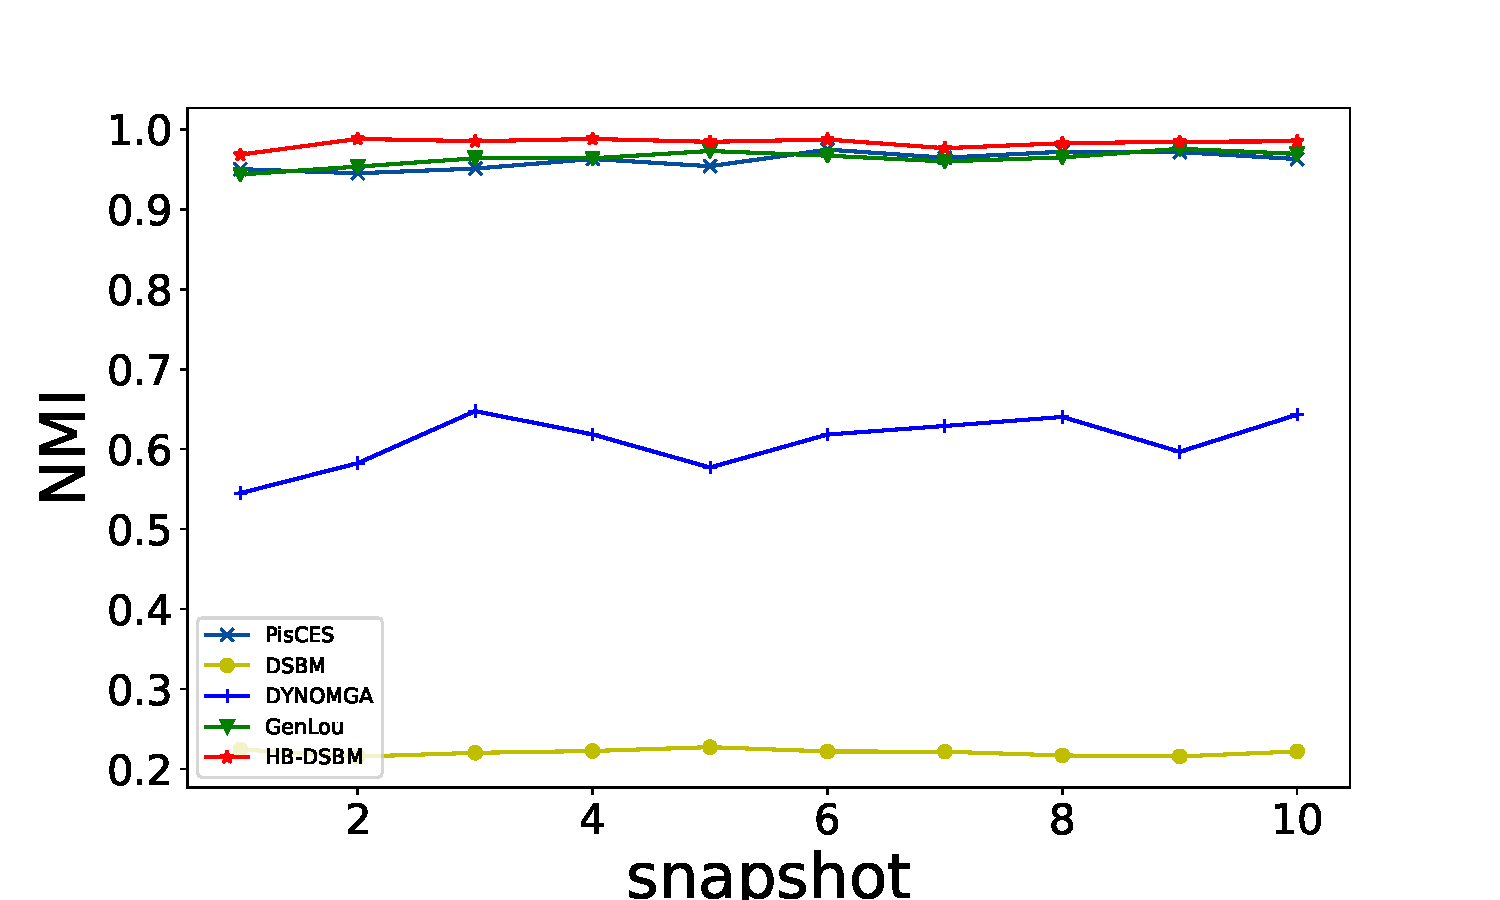
\includegraphics[width=.48\textwidth]{figures/chap04/swi1.pdf}
% 	}
% 	\caption{$data2$两个事件网络的不同方法NMI对比。}
% 	\label{fig.4.3}
% \end{figure}

% 真实世界数据集的实验如图~\ref{fig.4.4}~图\ref{fig.4.5}(a)所示,分别为KIT-email数据及DBLP数据。如图~\ref{fig.4.4}所示,HB-DSBM在KIT-email数据集中的NMI表现均高于其余方法,证明HB-DSBM不仅在生成数据集中具有较好表现,在真实世界数据集中也具有很好的社团检测效果。这里要强调的一点是,HB-DSBM在$t=1$的时候,效果并不比其余方法具有明显提升,因为HB-DSBM的改进主要注重在动态社团检测中节点的多层次演化,因此在第一个网络快照中的效果并不明显,而随着$t$的增长,HB-DSBM的效果会越来越好。




% \begin{figure}[htbp]
% 	\centering
% 	\subfigure[以两个月为间隔划分快照的网络]{
% 		% \label{Fig.vis.1}
% 		\label{fig.4.4.a}
% 		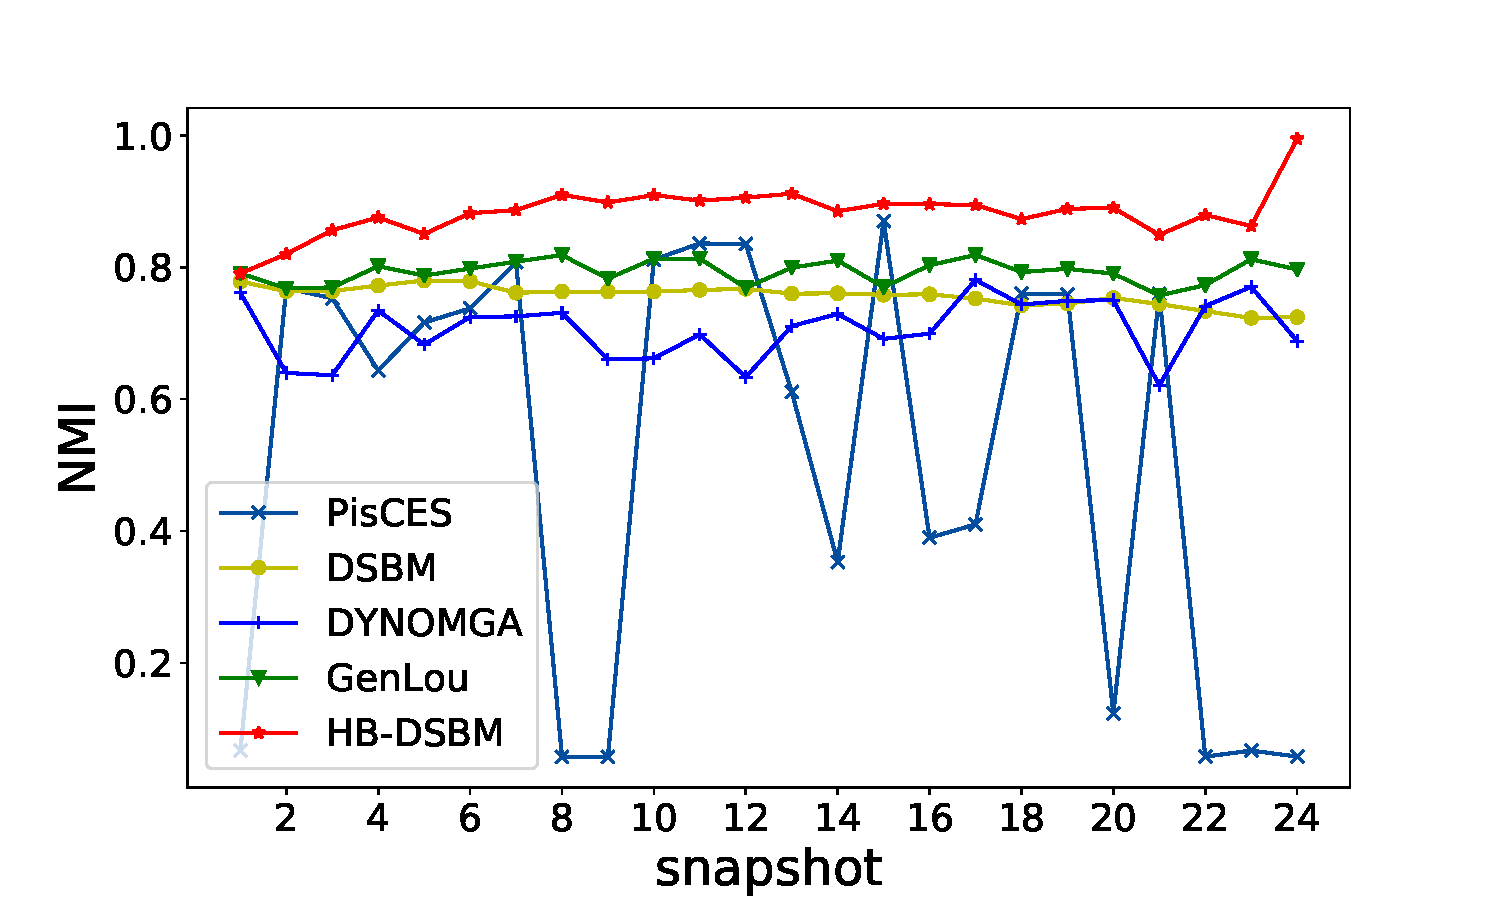
\includegraphics[width=.48\textwidth]{figures/chap04/compareInter2t.pdf}
% 	}
% 	\subfigure[以三个月为间隔划分快照的网络]{
% 		% \label{Fig.vis.1}
% 		\label{fig.4.4.b}
% 		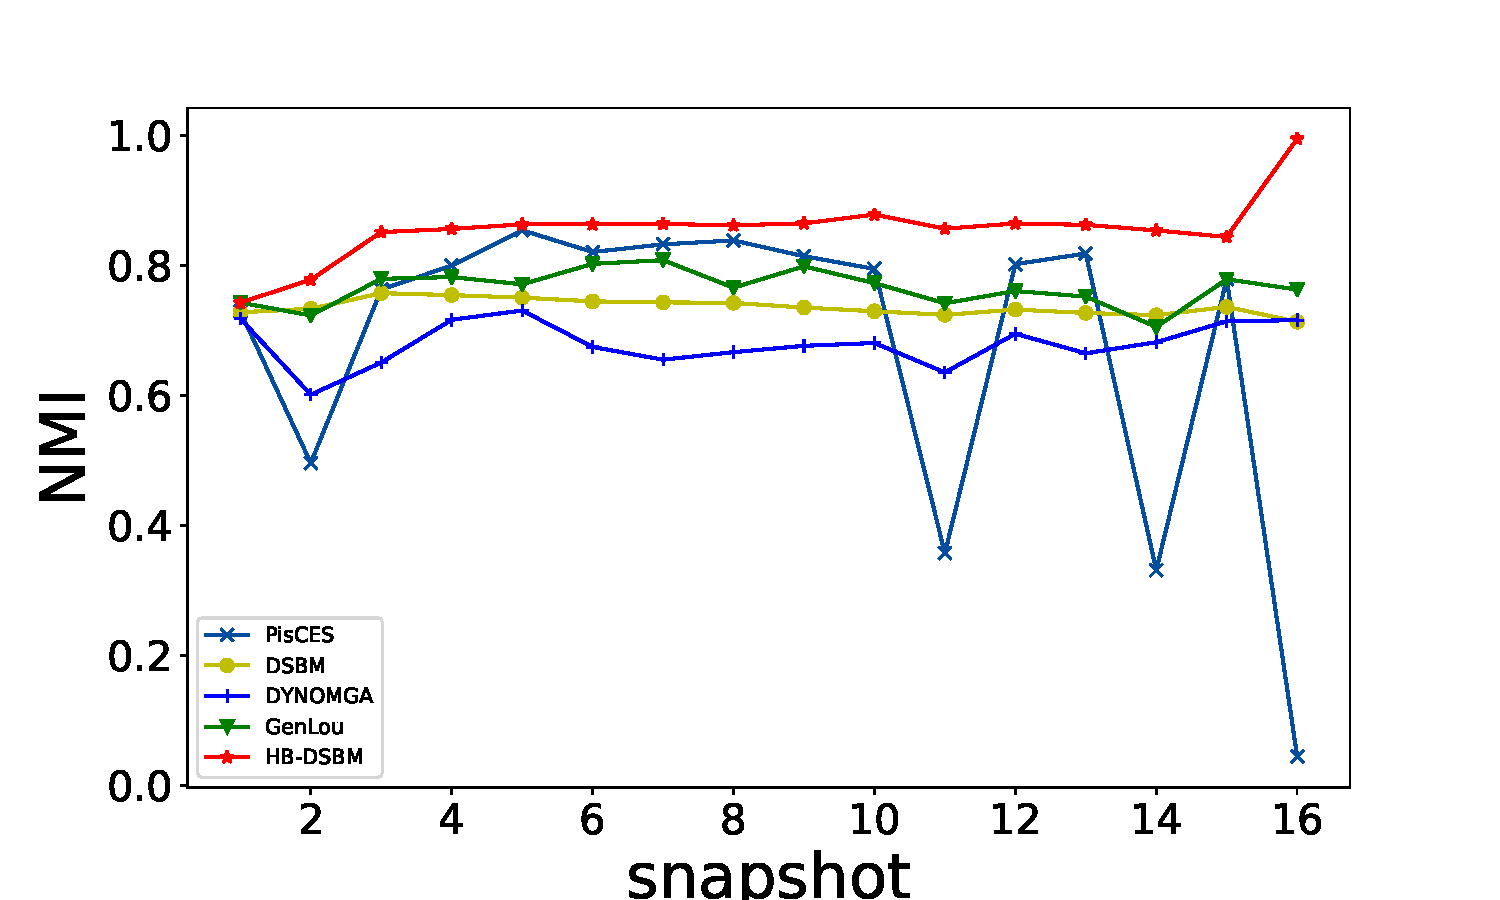
\includegraphics[width=.48\textwidth]{figures/chap04/compareInter3.pdf}
% 	}
% 	\caption{KIT-email数据不同时间间隔划分的切片网络的不同方法NMI对比}
% 	\label{fig.4.4}
% \end{figure}


% 而DBLP数据的同类方法对比如图\ref{fig.4.5}(a)所示,HB-DSBM的效果明显高于其他方法,再次证明了本模型的有效性。而DSBM的效果也优于其他方法,因为DSBM为生成模型,其同时融合了不同网络快照的社团检测与社团演化。而PisCES的噪声敏感性使得其在DBLP数据中的表现非常差,将所有节点划分到了同一个社团中。该数据集的不同方法NMI对比也再次证明了本文提出的动态网络社团演化层次贝叶斯结构的有效性。

% \begin{figure}[htbp]
% 	\centering
% 	\subfigure[DBLP数据的NMI对比]{
% 		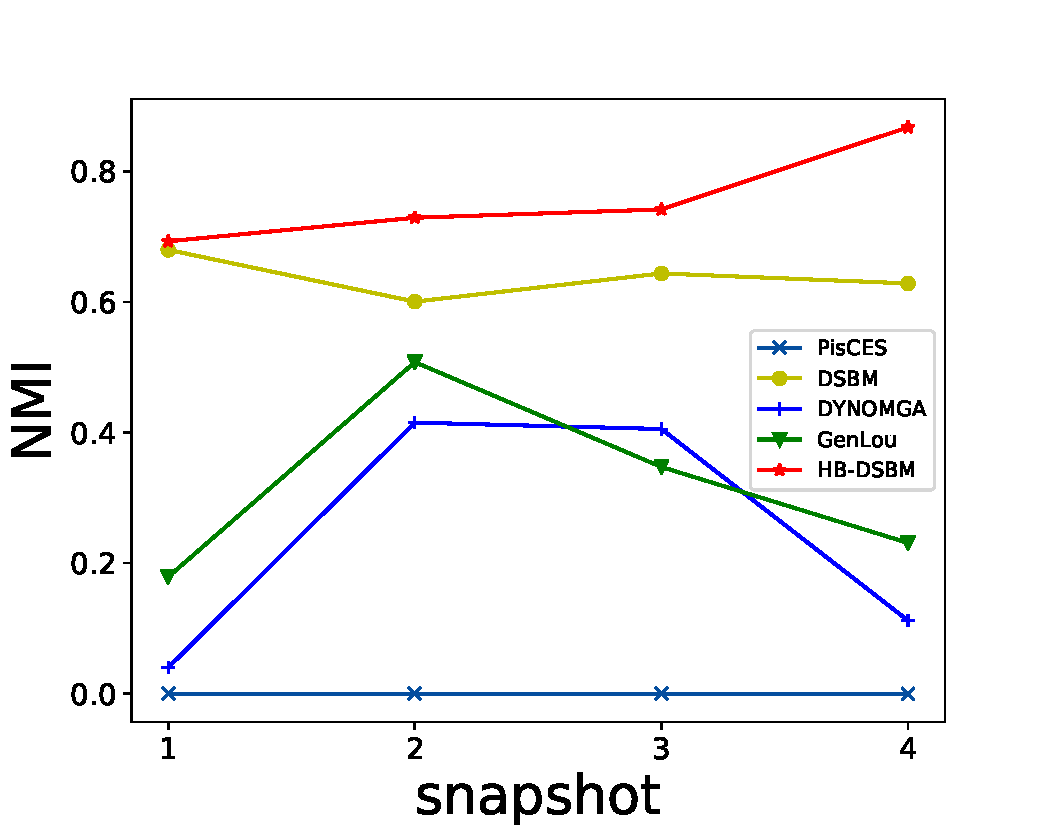
\includegraphics[width=.48\textwidth]{figures/chap04/dblp_t6789.pdf}
% 		\label{Fig.4.5.a}
% 	}
% 	\subfigure[DBLP以及$data1$的社团转移矩阵可视化]{
% 		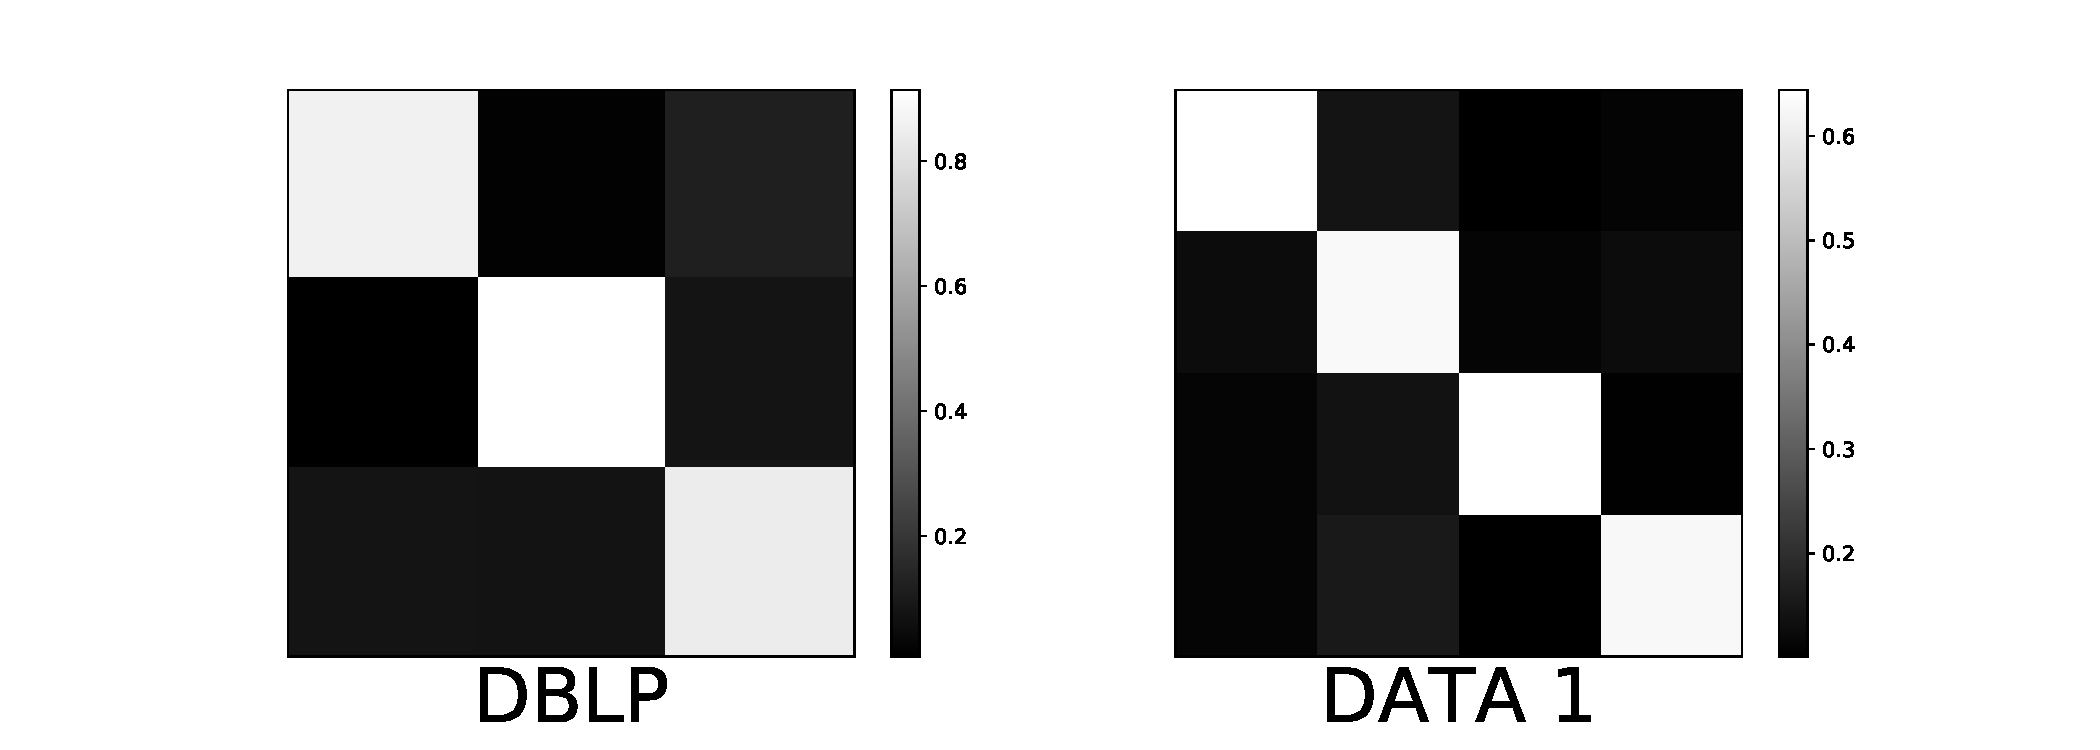
\includegraphics[width=.48\textwidth]{figures/chap04/communityHeatMap.pdf}
% 		\label{Fig.4.5.b}
% 	}
% 	\caption{DBLP数据社团检测及演化效果图。}
% 	\label{fig.4.5}
% \end{figure}


% \subsection{社团演化分析}

% 以往的模型如DSBM将在同一个社团的节点视作等价,也就是说在同一个社团的两个节点在模型中没有任何差别,它们具有相同的社团转移倾向,并且DSBM中的社团转移倾向矩阵并不会随着时间推移而变化。也就是说,以往的模型只考虑了节点的社团级别的演化倾向,并且是不变的。在HB-DSBM中,隐变量$C$和$A$分别代表了节点级别和社团级别的演化倾向,同时通过层次生成结构将这两个参数整合到了一起。模型社团级别的转移倾向矩阵$A$的可视化如图\ref{fig.4.5}(b)所示,图中分别展示了DBLP和$data1$的社团级别的转移倾向。然而社团级别的转移倾向并不是一成不变的,社团级别的转移倾向会随着时间变化,如图\ref{fig.4.6}可以看到,HB-DSBM准确把握住了不同网络快照中的社团级别的节点社团转移倾向。

% \begin{figure}[htbp]
% 	\centering
% 	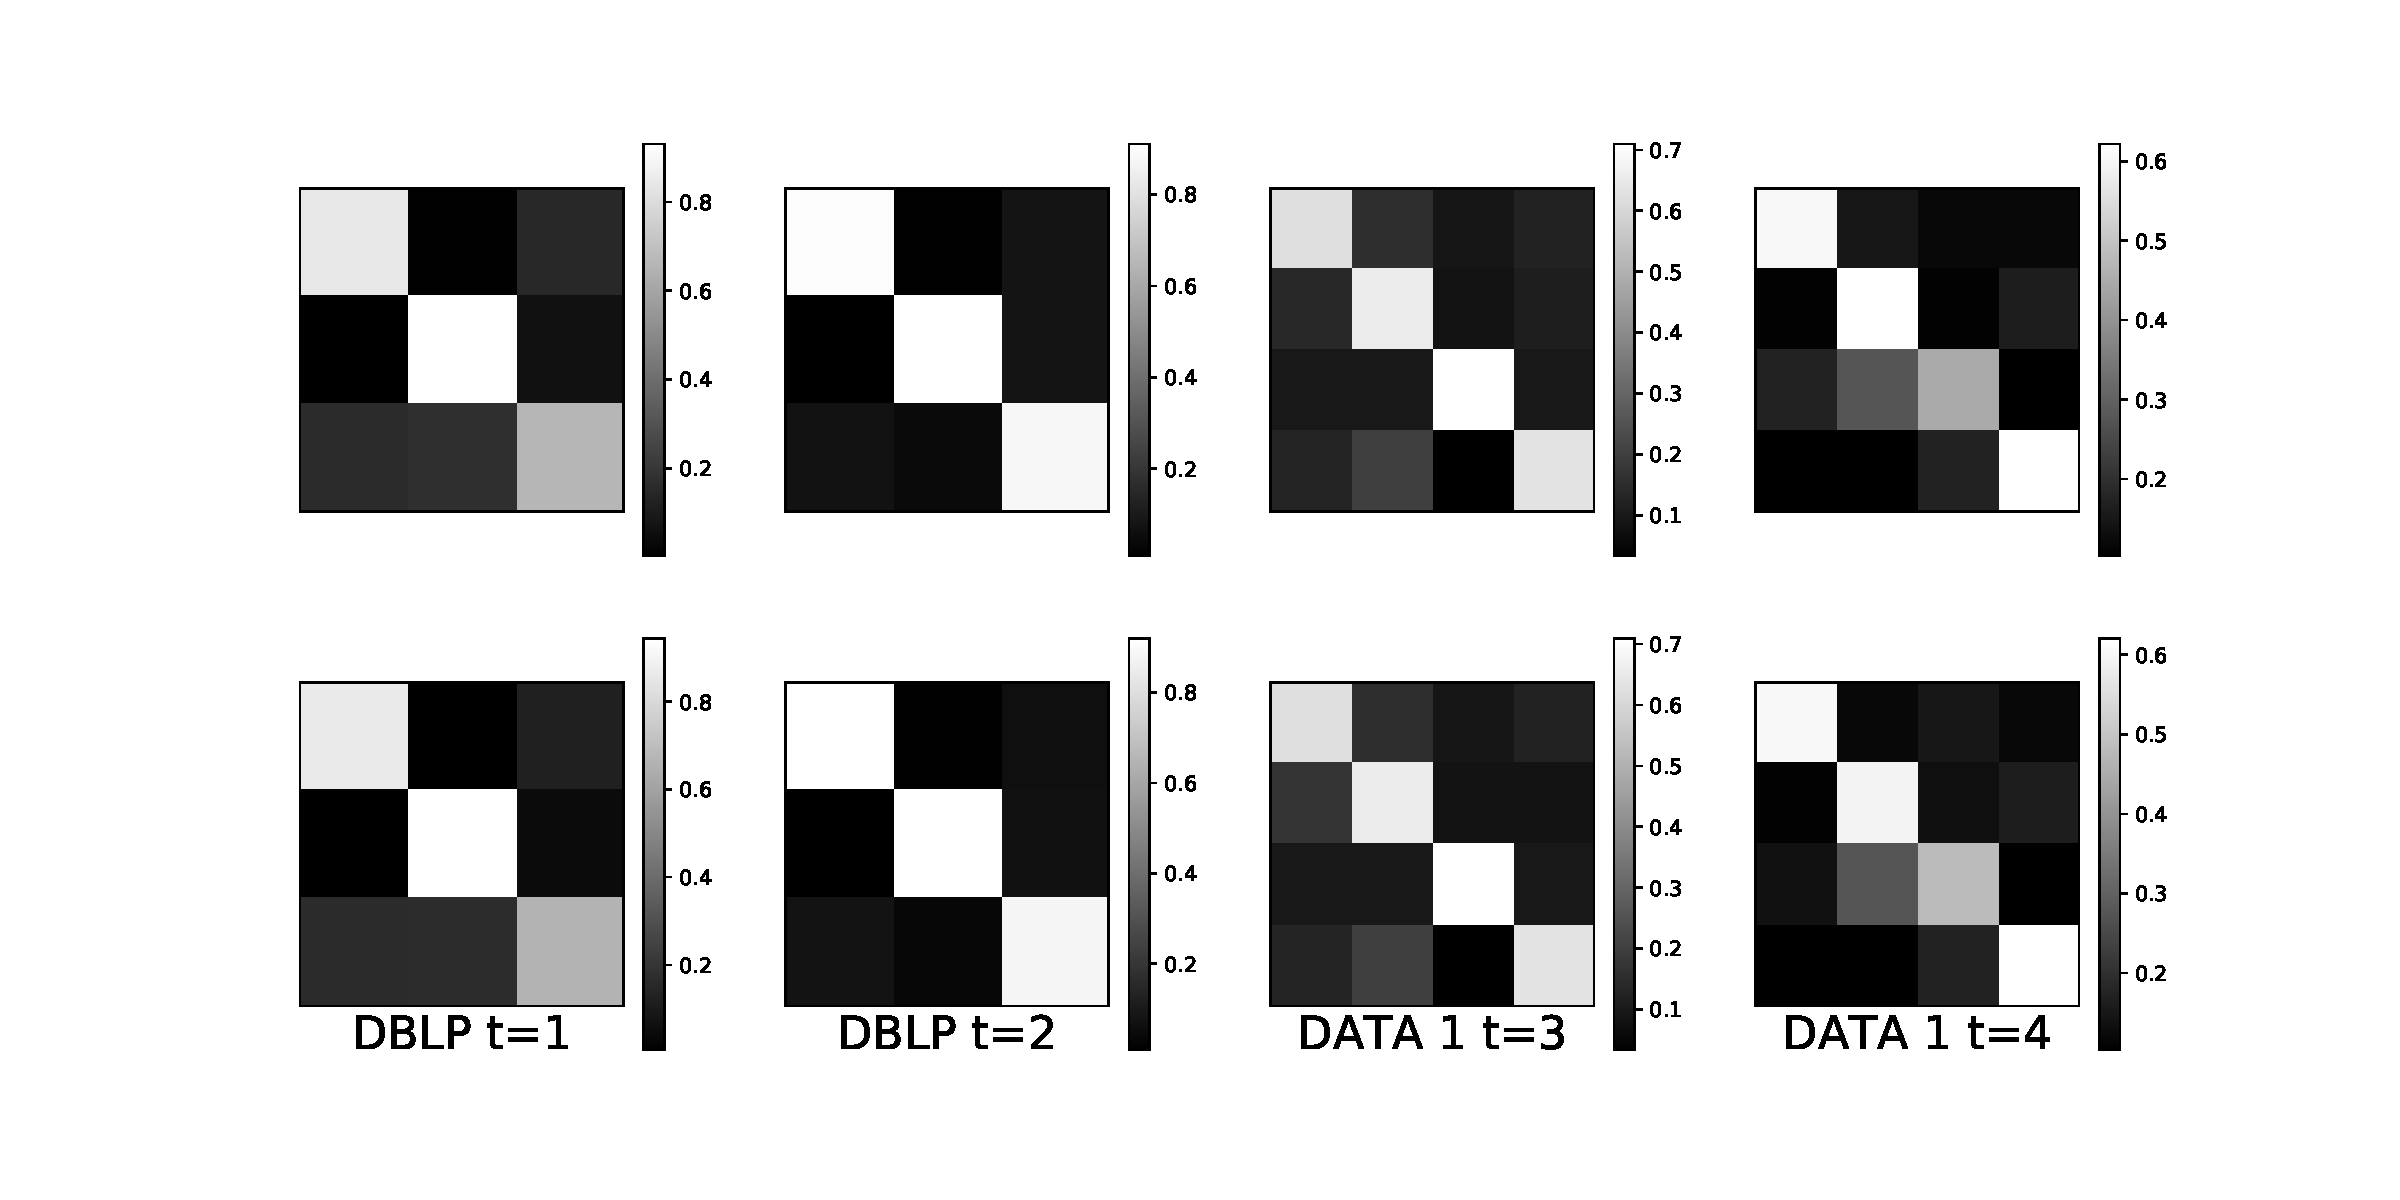
\includegraphics[width=.8\textwidth]{figures/chap04/communityHeatMapt.pdf}
% 	\caption{基于HB-DSBM模型的社团级别转移矩阵$A$分别在DBLP和$data1$数据的可视化(上半部分)与真实社团转移真相的可视化(下半部分)之间的对比。}
% 	\label{fig.4.6}
% \end{figure}


% 而同一社团的节点也具有不同的社团转移倾向,图\ref{fig.4.7}展示了DBLP数据中不同研究领域的作者的研究兴趣领域发生转移的倾向的异质性。例如,$Theo Gevers$在$2009$年发表了一篇数据挖掘的论文。根据模型的节点转移矩阵的计算,他有很大的倾向继续在数据挖掘领域发表论文,而事实也验证了模型的推算。
% \begin{figure*}[htbp]
% 	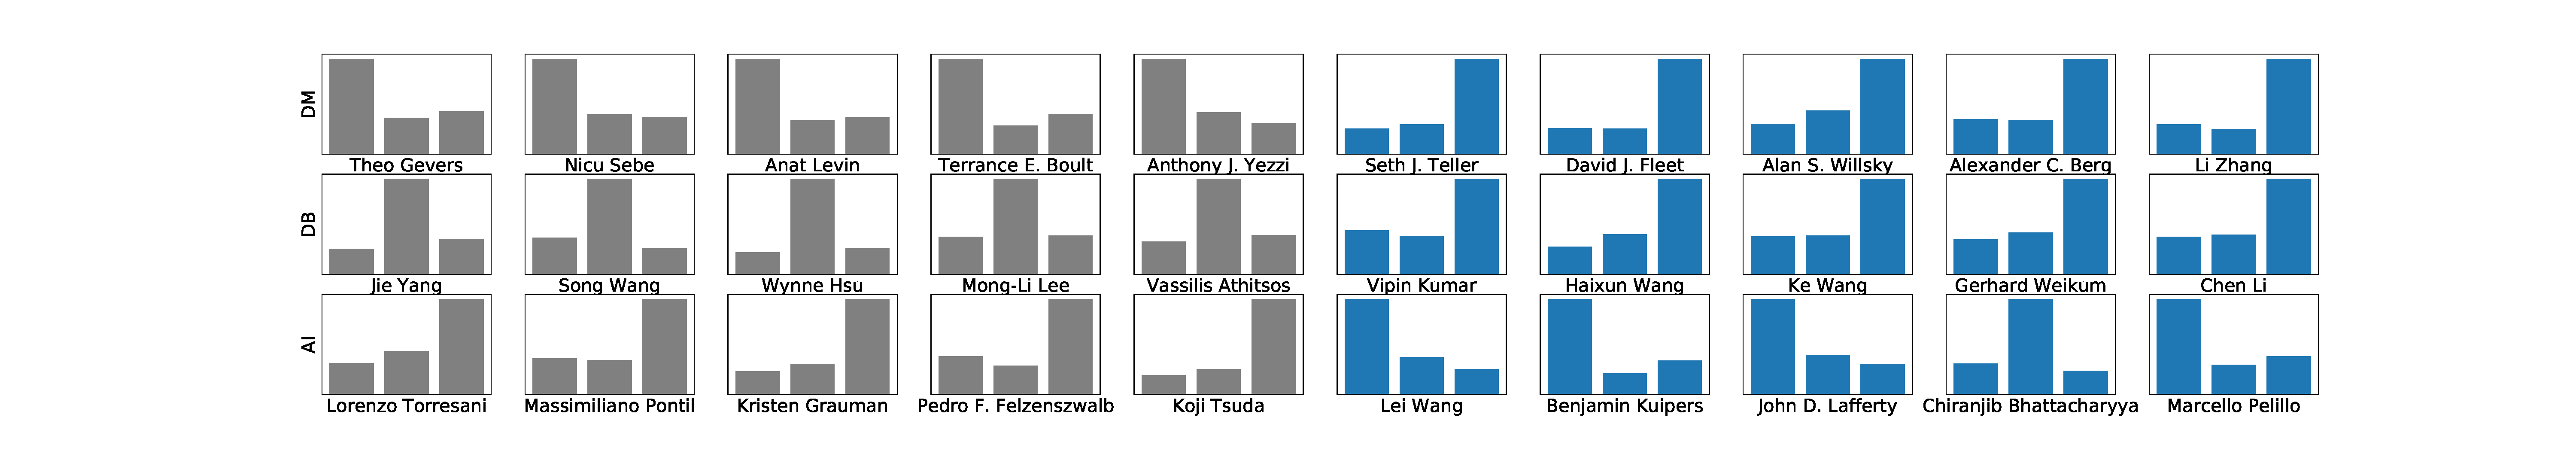
\includegraphics[width=\textwidth]{figures/chap04/nodes_compare.pdf}
% 	\caption{DBLP数据集中部分节点($2009-2010$年)的社团转移倾向可视化(基于节点级别转移倾向参数$C$)。每个柱状图代表一个节点的转移倾向,从左到右分别为DM,DB,AI。所有柱状图共三行,每行代表一个领域,从上到下分别为DM,DB,AI。灰色的柱状图代表节点社团转移倾向与其所在社团转移倾向一致,而蓝色的柱状图代表节点的转移倾向与其所在社团的转移倾向不一致。}
% 	\label{fig.4.7}
% \end{figure*}

% 通过HB-DSBM对DBLP数据的分析,本文还发现了一个有趣的现象,即大部分作者都倾向于在几年之内转换他们的研究兴趣领域。换句话说,只有很少一部分的作者会长期停留在同一个研究领域。如图\ref{fig.4.8}所示,$Svetlana Lazebnik$倾向于每两年转换一次研究兴趣领域,而这个时间间隔对$Jing Peng$来说则为三年。同时$Andrew W. Fitzgibbon$从数据挖掘在$t=7$时将研究领域转移到了人工智能领域。$Amnon Shashua$则将研究兴趣领域从人工智能转移到数据挖掘进行研究,四年后又将研究兴趣领域转移回了人工智能。

%  \begin{figure}[htbp]
%  	\centering
% 	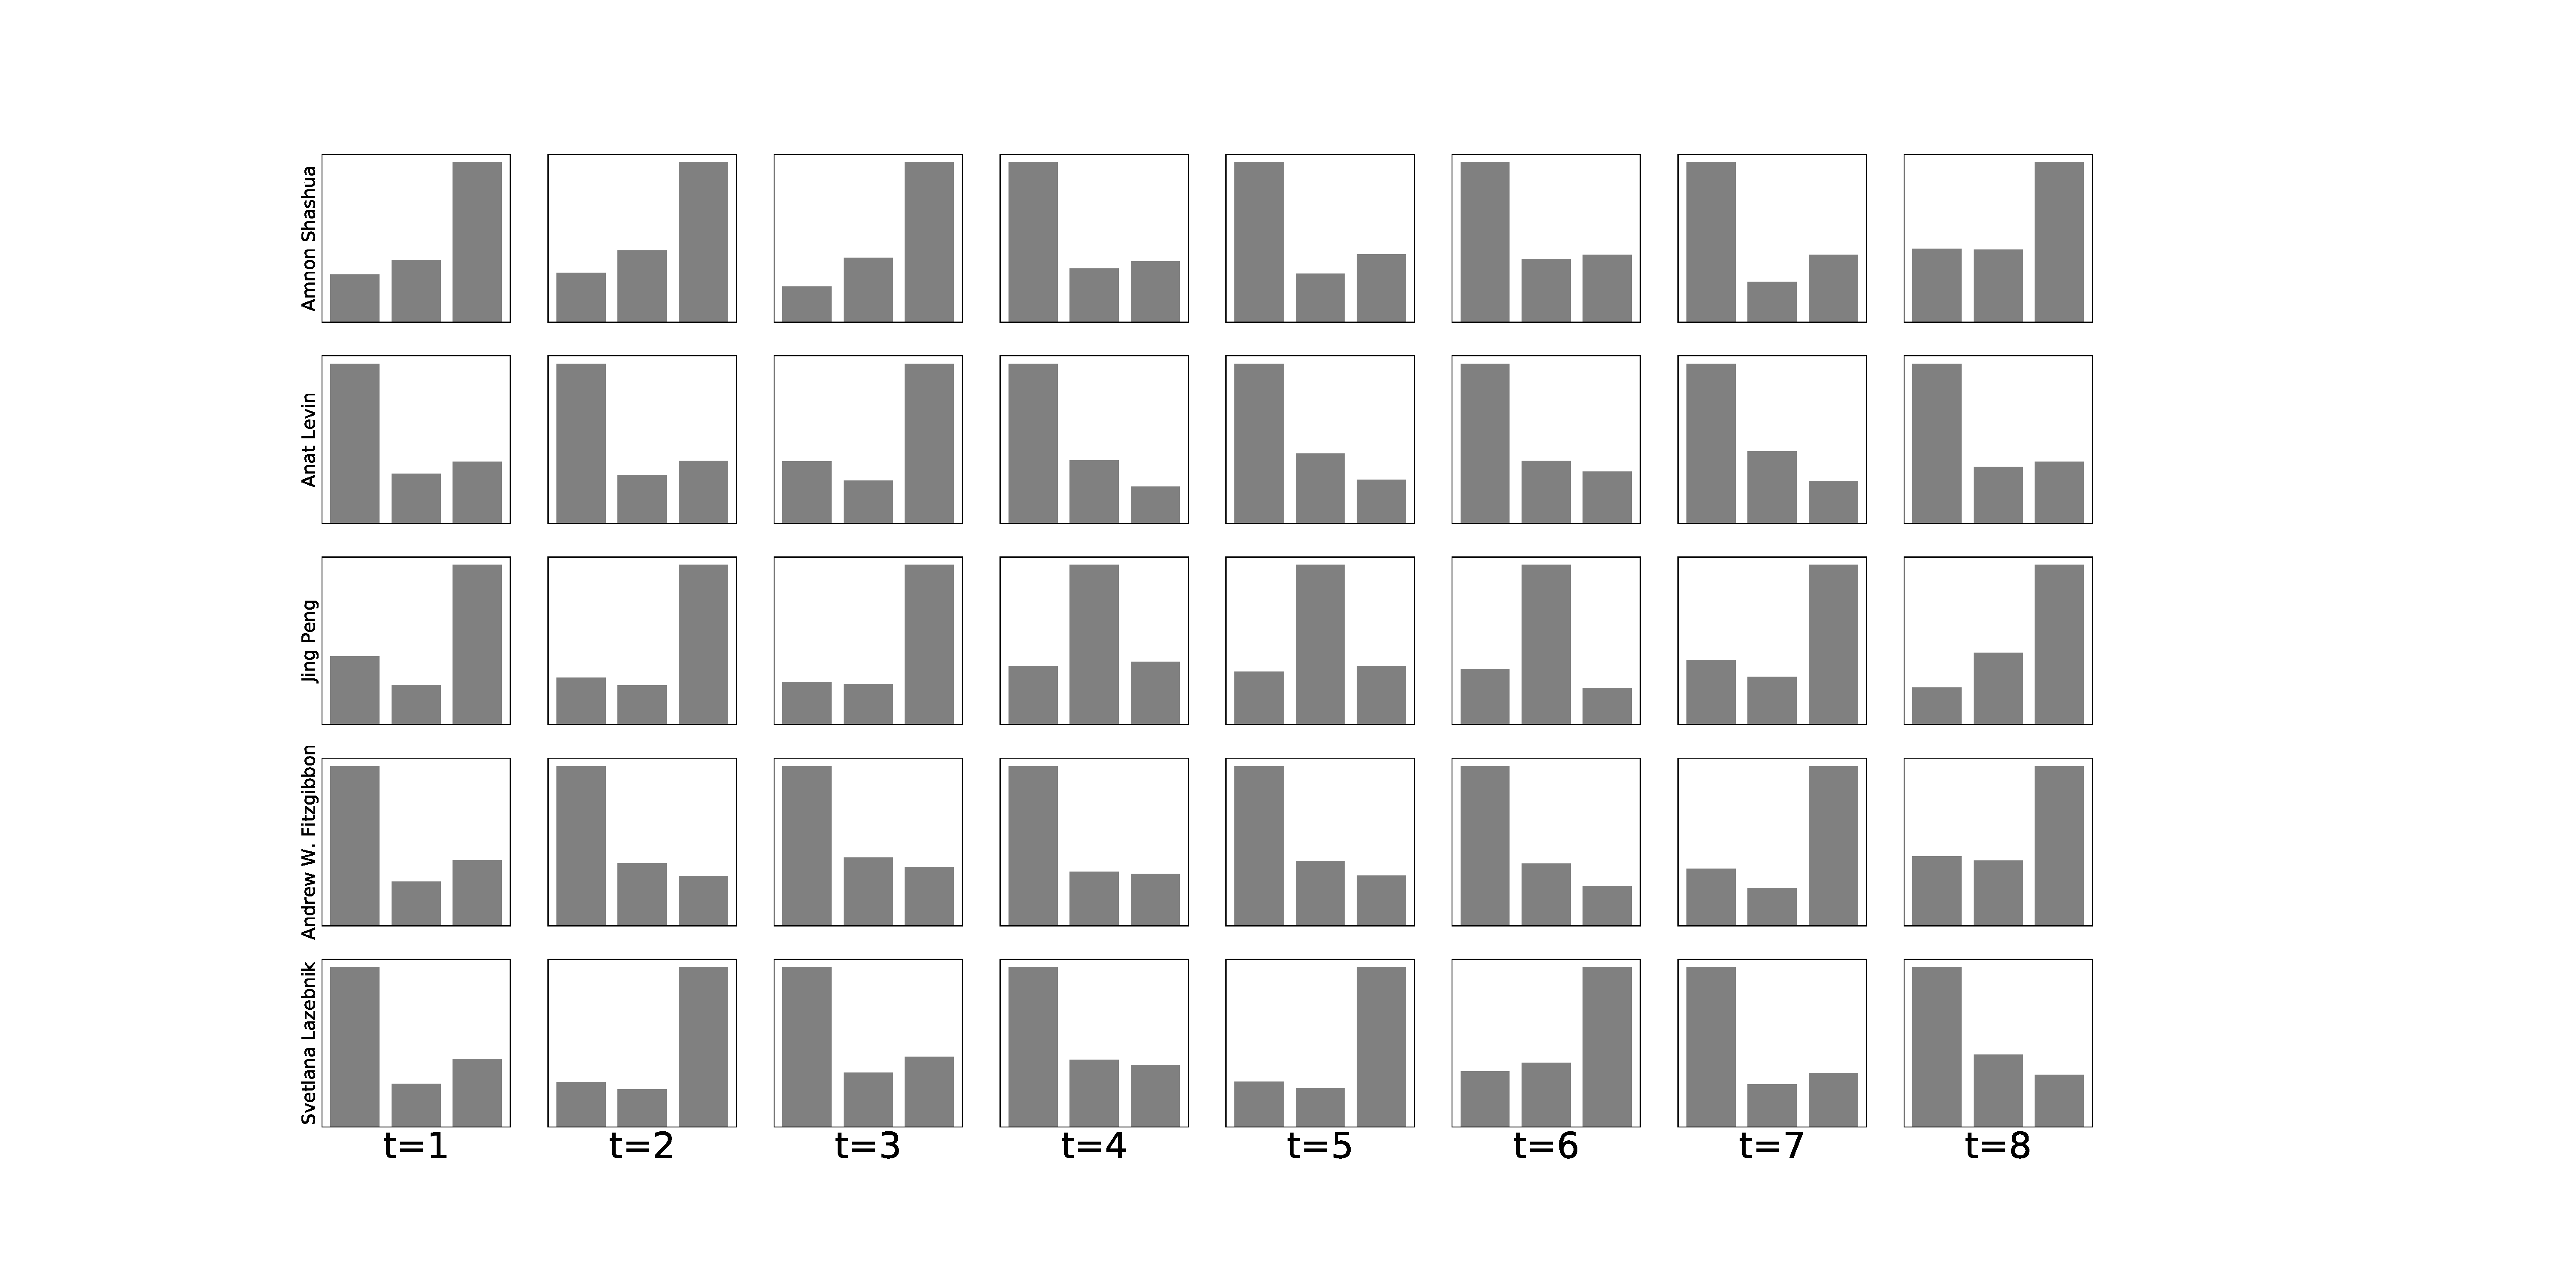
\includegraphics[width=.9\textwidth]{figures/chap04/nodes_evoluton1.pdf}
% 	\caption{DBLP数据选取的五个作者($Amnon Shashua, Anat Levin, Jing Peng, Andrew  W. Fitzgibbon, Svetlana Lazebnik$)的$8$年的转移倾向可视化。每个柱状图代表作者的社团转移倾向矩阵,从左到右分别为DM,DB,AI。}
% 	\label{fig.4.8}
% \end{figure}

% 为了衡量HB-DSBM在大数据集上的处理能力,本文将HB-DSBM和几个经典方法的运行效率进行了对比。数据集由著名的Dynamic Gervain Newman生成图算法进行生成,每个数据集有两个时间片,每个时间片具有不同的节点。图~\ref{fig.4.9}展示了HB-DSBM与对比方法在不同节点数据集上的运行时间的对比,图中可以看到,随着节点数的增加,PisCES与DSBM的计算用时超越了其他算法,效率变得很慢。值得一提的是,PisCES在每个时间片节点个数为$8192$时用时最长的同时,算法超过了最大迭代次数未收敛。而加入了随机采样模块后,变分推断结合随机采样的HB-DSBM随着节点数的增加,计算时间逐渐低于DSBM。可以看到,HB-DSBM的计算耗时曲线基本为线性增长,因此对于大规模数据集具有一定的处理能力。而PisCES与DSBM则接近于指数增长。运行速度最短的算法包括DYNMOGA与Genlouvain方法,而实际上,Genlouvain方法在对节点数为$8192$的动态网络进行社团检测时,由于内存不足导致了算法异常终止(Linux系统$16$G内存)。因此Genlouvain算法在实际使用时需要具有足够大的内存。而DYNMOGA算法使用了多目标优化的策略对动态网络进行社团检测,这种策略使得其算法可以多点并行,因而其运行速度凌驾于其他算法之上。受此启发,HB-DSBM也可以在后期加入并行计算,以此来进一步提升算法的运行效率。

%  \begin{figure}[htbp]
% 	\centering
% 	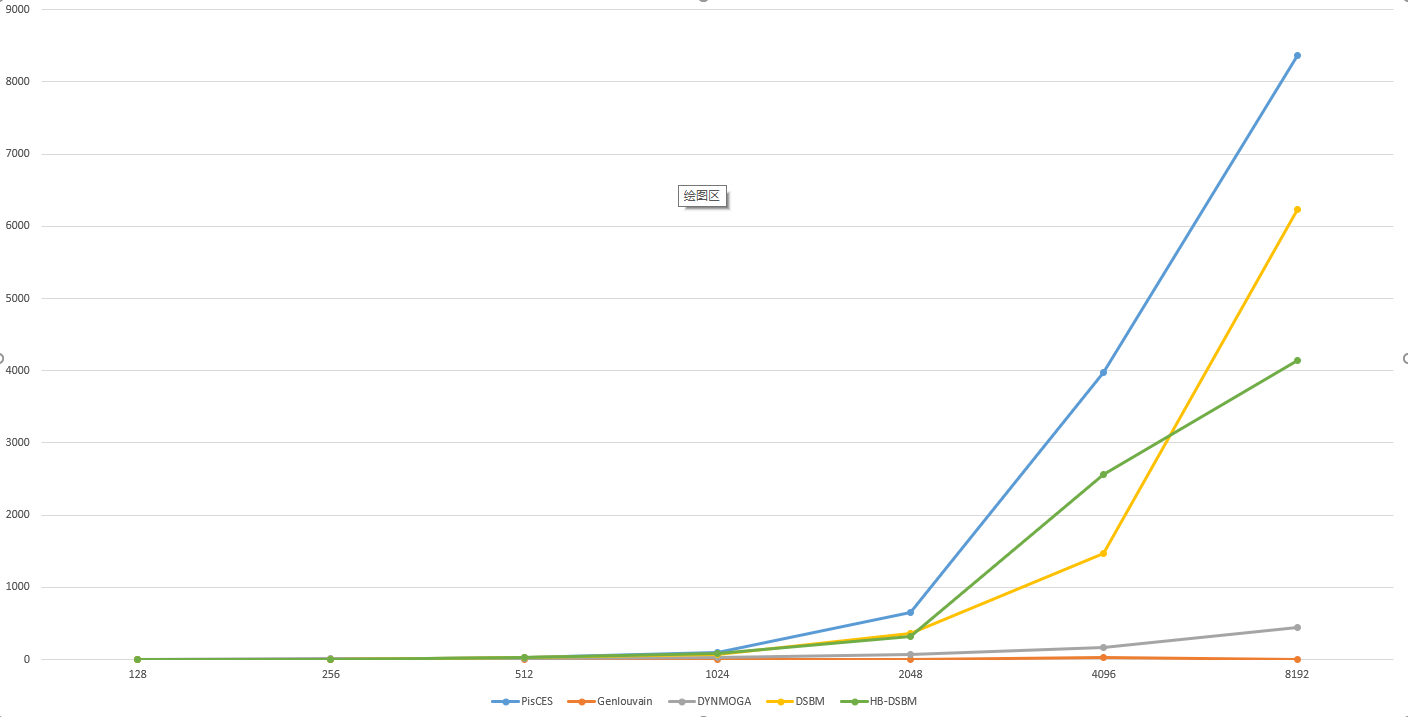
\includegraphics[width=.9\textwidth]{figures/chap04/performance.png}
% 	\caption{HB-DSBM与baseline方法在不同节点数的动态网络中的运行时间对比,横坐标为节点数,纵坐标为运行时间(s)。}
% 	\label{fig.4.9}
% \end{figure}

% \section{本章小结}
% 本章介绍了层次贝叶斯动态随机块模型,其层次贝叶斯生成结构能够同时融合节点级别以及社团级别的社团演化模式。同时本文利用变分推断对模型参数进行估计,利用合理的优化策略,模型可以适应大规模数据的计算。同类方法的对比也显示出HB-DSBM在动态网络社团检测任务中更加高效准确。

